\documentclass[output=book,nonflat,modfonts,
  colorlinks,citecolor=brown, 
 draft,draftmode,  
%  showindex,
%  nobabel,
%  booklanguage=german,
%  multiauthors,
		  ]{langsci/langscibook}    
  
%%%%%%%%%%%%%%%%%%%%%%%%%%%%%%%%%%%%%%%%%%%%%%%%%%%% 
%%%          additional packages                 %%% 
%%%%%%%%%%%%%%%%%%%%%%%%%%%%%%%%%%%%%%%%%%%%%%%%%%%% 

\author{Sonia Ben Hedia} %look no further, you can change those things right here.
\title{Gemination and degemination in English affixation}  
\subtitle{Investigating the interplay between morphology, phonology and phonetics}
%\BackTitle{Change your backtitle in localmetadata.tex} % Change if BackTitle is different from Title

\renewcommand{\lsSeries}{silp} % use lowercase acronym, e.g. sidl, eotms, tgdi
\renewcommand{\lsSeriesNumber}{99} %will be assigned when the book enters the proofreading stage

\BackBody{In English, phonological double consonants only occur across morphological boundaries, for example, in affixation (e.g. in \textit{unnatural}, \textit{innumerous}). There are two possibilities for the phonetic realization of these morphological geminates: Either the phonological double is realized with a longer duration than a phonological singleton (gemination), or it is of the same duration as a singleton consonant (degemination). 
	
The present book provides the first large-scale empirical study on the gemination with the five English affixes \textit{un}-, locative \textit{in}-, negative \textit{in}-, \textit{dis}- and –\textit{ly}. Using corpus and experimental data, the predictions of various approaches to the morpho-phonological and the morpho-phonetic interface are tested. By finding out which approach can account best for the gemination pattern of English affixed words, important implications about the interplay between morphology, phonology and phonetics are drawn.}

%\dedication{Change dedication in localmetadata.tex}
%\typesetter{Change typesetter in localmetadata.tex}
%\proofreader{Change proofreaders in localmetadata.tex}

\renewcommand{\lsID}{221} % contact the coordinator for the right number
%\BookDOI{}%ask coordinator for DOI
\renewcommand{\lsISBNdigital}{000-0-000000-00-0}
\renewcommand{\lsISBNhardcover}{000-0-000000-00-0} 

% add all extra packages you need to load to this file  
\usepackage{tabularx} 
\usepackage{tabu} % tabellen an die Seiten anpassen
\usepackage{longtable}
\usepackage{multicol}
\usepackage{array}
\usepackage{multirow}
% \usepackage{adjustbox}
\usepackage{appendix}

\usepackage{listings}
\lstset{basicstyle=\ttfamily,tabsize=2,breaklines=true}


% \usepackage{graphicx} % to include graphs 
\graphicspath{ {images/} } %my path in which I store the graphs

\usepackage{subfigure} % so kann man subfigzres macehn
%\usepackage{subcaption}

\usetikzlibrary{shapes,arrows,positioning,fit}
\usetikzlibrary{backgrounds}
\usepackage{tikz-qtree}

% % \usepackage[safe]{tipa} % IPA
\usepackage{latexsym} % Sonderzeichen

\usepackage{csquotes}

%%%%%%%%%%%%%%%%%%%%%%%%%%%%%%%%%%%%%%%%%%%%%%%%%%%%
%%%                                              %%%
%%%           Examples                           %%%
%%%                                              %%%
%%%%%%%%%%%%%%%%%%%%%%%%%%%%%%%%%%%%%%%%%%%%%%%%%%%% 
%% to add additional information to the right of examples, uncomment the following line
% \usepackage{jambox}
%% if you want the source line of examples to be in italics, uncomment the following line
% \renewcommand{\exfont}{\itshape}
\usepackage{./langsci/styles/langsci-optional}
\usepackage{./langsci/styles/langsci-lgr}
\makeatletter
\let\pgfmathModX=\pgfmathMod@
\usepackage{pgfplots,pgfplotstable}%
\let\pgfmathMod@=\pgfmathModX
\makeatother
\usepackage{./langsci/styles/langsci-gb4e}

%% hyphenation points for line breaks
%% Normally, automatic hyphenation in LaTeX is very good
%% If a word is mis-hyphenated, add it to this file
%%
%% add information to TeX file before \begin{document} with:
%% %% hyphenation points for line breaks
%% Normally, automatic hyphenation in LaTeX is very good
%% If a word is mis-hyphenated, add it to this file
%%
%% add information to TeX file before \begin{document} with:
%% %% hyphenation points for line breaks
%% Normally, automatic hyphenation in LaTeX is very good
%% If a word is mis-hyphenated, add it to this file
%%
%% add information to TeX file before \begin{document} with:
%% \include{localhyphenation}
\hyphenation{
affri-ca-te
affri-ca-tes 
}

\hyphenation{
Ha-nique
}

\hyphenation{
whe-ther
}

\hyphenation{
Relative-Frequency
Rela-tiveFrequency
}

\hyphenation{
Type-OfBase
TypeOf-Base
}


\hyphenation{
over-view
}

\hyphenation{
initial-strengthen-ing
}
\hyphenation{
Semantic-Transparency
SemanticTrans-parency
}

\hyphenation{
morpho-pho-nology
mor-pho-phonology
}

\hyphenation{
Semantic-TransparencyRating
SemanticTransparency-Rating
}
\hyphenation{
affri-ca-te
affri-ca-tes 
}

\hyphenation{
Ha-nique
}

\hyphenation{
whe-ther
}

\hyphenation{
Relative-Frequency
Rela-tiveFrequency
}

\hyphenation{
Type-OfBase
TypeOf-Base
}


\hyphenation{
over-view
}

\hyphenation{
initial-strengthen-ing
}
\hyphenation{
Semantic-Transparency
SemanticTrans-parency
}

\hyphenation{
morpho-pho-nology
mor-pho-phonology
}

\hyphenation{
Semantic-TransparencyRating
SemanticTransparency-Rating
}
\hyphenation{
affri-ca-te
affri-ca-tes 
}

\hyphenation{
Ha-nique
}

\hyphenation{
whe-ther
}

\hyphenation{
Relative-Frequency
Rela-tiveFrequency
}

\hyphenation{
Type-OfBase
TypeOf-Base
}


\hyphenation{
over-view
}

\hyphenation{
initial-strengthen-ing
}
\hyphenation{
Semantic-Transparency
SemanticTrans-parency
}

\hyphenation{
morpho-pho-nology
mor-pho-phonology
}

\hyphenation{
Semantic-TransparencyRating
SemanticTransparency-Rating
}
\addbibresource{gem.bib}

%%%%%%%%%%%%%%%%%%%%%%%%%%%%%%%%%%%%%%%%%%%%%%%%%%%% 
%%%             Frontmatter                      %%% 
%%%%%%%%%%%%%%%%%%%%%%%%%%%%%%%%%%%%%%%%%%%%%%%%%%%% 
\begin{document}  
\input{localcommands.tex} 
  
\maketitle                
\frontmatter 

\currentpdfbookmark{Contents}{name} % adds a PDF bookmark
{\sloppy\tableofcontents}
 %\include{chapters/preface}
%  \include{chapters/acknowledgments}
 %\include{chapters/abbreviations} 
\mainmatter     
 
%%%%%%%%%%%%%%%%%%%%%%%%%%%%%%%%%%%%%%%%%%%%%%%%%%%% 
%%%             Chapters                         %%% 
%%%%%%%%%%%%%%%%%%%%%%%%%%%%%%%%%%%%%%%%%%%%%%%%%%%%

 %add a percentage sign in front of the line to exclude this chapter from book
 \chapter{Introduction} \label{Introduction}



%Gemination: what is it. Morpho-phonolo pehneomeonen
In English, affixation may lead to the adjacency of two identical consonants across a morpheme boundary. When in a derivative the final consonant of the prefix and the first consonant of the base are the same, a phonological double consonant emerges (see examples \ref{example gemination un} --\ref{example gemination dis}). The same happens when the first consonant of the suffix and the last consonant of the base are the same (see example \ref{example gemination ly}). I will call these phonological double consonants \newterm{morphological geminates}.


\begin{exe} 
	\ex \label{example gemination un} \textbf{\prefix{un}:} \hspace*{1cm}\prefix{un}\textit{natural}, \prefix{un}\textit{known}
	\ex \label{example gemination in} \textbf{\prefix{in}:} \hspace*{1cm} \prefix{in}\textit{numerous}, \prefix{im}\textit{mortal}
	\ex \label{example gemination dis} \textbf{\prefix{dis}:}  \hspace*{1cm}\prefix{dis}\textit{satisfy}, \prefix{dis}\textit{solution}
	\ex \label{example gemination ly} \textbf{\suffix{ly}:}  \hspace*{1.2cm}\textit{real}\suffix{ly}, \textit{sole}\suffix{ly}
\end{exe}

 There are two possibilities for the phonetic realization of morphological geminates: Either the phonological double is realized with a longer duration than a phonological singleton (gemination), or it is of the same duration as a singleton consonant (degemination). It is, however, yet unclear in which cases we find gemination, and in which we find degemination.
 
%Not much investigated but just claims are made
There are numerous claims about the pattern of gemination in English affixation in the literature (see, for example, \citealt[141]{Wijk.1966}; \citealt[255]{OConnor.1973}; \citealt[18]{Mohanan.1986}; \citealt[251]{Ladefoged.1993}; \citealt{Roach.2011,Wells.2008}; \citealt[1055 f.]{CohenGoldberg.2013}), but there is hardly any evidence for these claims. %Large-scale empirical research on gemination in English has been lacking. 
Only four studies have empirically investigated gemination in English affixed words: \cite{Kaye.2005}, \cite{Oh.2012}, \cite{Oh.2013} and \cite{Kotzor.2016}. Due to methodological issues and the small scale of the studies, their empirical findings are not sufficient to explain the gemination pattern of English affixational geminates.



%Beause it is a morpho-phonolo phenomoen spanning morph bundaries very well suited to investigate the interface
As gemination in English affixation can be regarded as a morpho-phonological process which is mirrored on the phonetic level, explaining its pattern is of high theoretical importance for morpho-phonological approaches which discuss the role of phonetics in phonology and morphology. Finding out which factors govern gemination in English affixation can reveal important insights about the interplay between morphology, phonology and phonetics.

% The theoires
One can distinguish between two major branches of morpho-phonological approaches. The first one can be categorized as rule based and  categorical in nature, while the second one is founded on the assumption that processes are gradient and dependent on the properties of individual words. 
Both types of approaches assume morphological boundary strength to affect the phonetic realization of complex words. 
It is generally assumed that weaker boundaries lead to more phonetic reduction, while stronger boundaries lead to less reduction. 
The two types of approaches deviate, however, in how they conceptualize these boundaries. In turn, they differ in their predictions about how morphological boundaries affect the phonetic realization of complex words, including the phonetic realization of morphological geminates.
 

Categorical approaches like Lexical Phonology (cf., for example, \citealt{Kiparsky.1982}, \citealt{Mohanan.1986}) assume boundary strength to depend on affixes. Affixes belong to different lexical strata which determine the phonological relation between an affix and its base. This relation is reflected on the phonetic level. 
For the phenomenon of gemination it is predicted that level 1 affixes, such as \prefix{in}, are separated from their base by a weak morphological boundary and hence degeminate. Level 2 affixes, such as \prefix{un}, in contrast geminate due to the strong morphological boundary which they feature. 

Gradient probabilistic approaches, on the other hand, would expect factors which are related to individual derivatives to govern gemination. The Morphological Segmentability Hypothesis (\citealt{Hay.2003}), for example, claims that the decomposability of a word determines the boundary strength between the affix and its base. This strength is assumed to be mirrored in phonetic detail, such as the duration and reduction of boundary adjacent segments. Applied to gemination, one would thus expect that more decomposable words display longer consonant durations (gemination), while less decomposable words display shorter durations (degemination). 


In this book, I will test the predictions for morphological gemination made by various approaches to the morpho-phonological and the morpho-phonetic interface. 
On the one hand, I will test the predictions made by formal linguistic theories, which are mostly categorical in nature. On the other, I will test predictions which are derived from psycholinguistic approaches, which are mostly gradient in nature. Furthermore, I will test some general assumptions about the realization of complex words, as proposed by different models of speech production.

I will investigate morphological gemination with the five English affixes \prefix{un}, negative \prefix{in}, locative \prefix{in}, \prefix{dis} and adverbial \suffix{ly}. The gemination pattern of each affix will be investigated in a corpus and an experimental study. 
By finding out which approach can account best for the gemination pattern of English affixed words, important implications about the interplay between morphology, phonology and phonetics can be drawn.


%Structure

The book is structured as follows.
 In chapter \ref{Gemination}, I will give an overview of the phenomenon \newterm{gemination}. I will introduce key terminology, discuss the phonological representation of geminates and summarize previous work on gemination. I will mainly focus on morphological gemination in English. 
 In chapter \ref{affixes}, I will turn to the five affixes investigated in this book. I will describe the characteristics of each affix and compare them in a qualitative analysis. 
  In  chapter \ref{Theory}, I will discuss the three investigated fields of morpho-phonological and morpho-phonetic approaches: Formal linguistic theories, psycholinguistic approaches to morphological processing and theories of speech production. I will summarize the main aspects of each field, discuss the most important theories in the field, and deduce the predictions each theory makes for gemination with the five affixes under investigation. 
  These predictions will then be tested in a corpus study and an experimental study. The studies will be discussed in chapters \ref{General Method}--\ref{Conclusion}.
   While in chapter \ref{General Method} the general methodology underlying both studies will be described, 
  chapter \ref{Corpus Studies} will focus on the methodology, analyses and results of the corpus study, and 
  chapter \ref{Experimental Studies} will focus on the methodology, analyses and results of the experimental study.
   In chapter \ref{Conclusion}, the results of both studies will be summarized and discussed with regard to the approaches discussed in chapter \ref{Theory}.
  In chapter \ref{final conclusion} a final conclusion will be given.\footnote{Earlier versions of parts of chapter \ref{Gemination}, chapter \ref{General Method} and chapter \ref{Corpus Studies} have been previously published in \cite{BenHedia.2017}. They were only minimally altered for the present book. The pertinent chapters and sections will be identified by a footnote.}




 
% \chapter{Gemination} \label{Gemination}


In this chapter, I will introduce and clarify the key terminology and notions necessary to understand the theoretical implications of this book. I will discuss different types of geminates and thereby show how gemination is a phonological as well as a morphological phenomenon. I will also explain the important role of phonetics in investigating gemination. After clarifying some general notions on gemination, I will concentrate on gemination in English by reviewing assumptions and previous research. 

\section{Geminates} \label{what is gemination}

Geminates are taken to be double consonants which are articulated with a particularly long duration (e.g. \citealt{Hartmann.1972, Catford.1988, Trask.1996, Matthews.1997, Crystal.2008,Davis.2011, Galea.2016}). Lexical (or `true') geminates denote a phonemic difference, i.e. they make up minimal pairs with their singleton counterparts such as in the Japanese words  \textit{kona} ‘powder’ versus \textit{konna} ‘such'. A second type of geminate are double consonants arising across a morphological boundary from the concatenation of two morphemes, such as in the English prefixed word \textit{unnatural} or the compound \textit{fun name}. For this type of geminates various labels are found in the literature, among them `fake' geminates (for example used by \citealt{Hayes.1986b}; \citealt{Oh.2012} and \citealt{Kotzor.2016}), derived geminates (for example used by \citealt{Kubozono.2017b}), concatenated geminates (for example used by \citealt{Ridouane.2010}) and surface geminates (for example used by \citealt{Lahiri.1988, Galea.2016}). I will refer to them as ‘morphological geminates'.


The main feature of geminates, distinguishing them from singletons, is their longer duration. But what is the durational difference between geminates and singletons? Acoustic research has shown that there is no universal answer to this question. The singleton-geminate ratio depends on various factors, such as the language of the geminate, the type of segment the geminate is made of and the geminate's position. With regard to cross-linguistic differences a review of empirical work on the topic reveals quite a big range of singleton-geminate ratios between languages.  Stop geminates in word-medial position are, for example, found to range from 1:1.5 in Madurese (\citealt{Cohn.1999}) to 1:2.9 in Turkish (\citealt{Lahiri.1988}) (see also \citealt[38 f.]{Dmitrieva.2017} for discussion of language-specific differences). 
Furthermore, durational differences heavily depend on the type of segment involved. For instance, \cite{Aoyama.2006} find that for Guinaang Bontok the highest ratios, i.e. the longest geminates, can be found with nasals (ratios between 1:1.72 and 1:2.15), followed by lateral approximants (ratio: 1:2.0), stops (ratios between 1:1.81 and 1:1.90), approximants (ratios between 1:1.56 and 1:1.69) and fricatives (ratio for [s]: 1:1.56). The lowest ratio is found for glides (ratio: 1:1.39). Similarly, for Italian,  \cite{Payne.2005} finds the longest geminates with nasals and laterals (ratio for nasals: 1:2.1, ratio for laterals: 1:2.3) and the shortest with fricatives (ratio: 1:1.5). 
 The influence of position is yet unclear and seems to depend on the language investigated (see \citealt[chapter 3]{Galea.2016} and \citealt[36 f.]{Dmitrieva.2017} for a discussion of cross-linguistic gemination in different positions). While \cite{Ridouane.2010}, for example, finds that word-final geminates are longer than word-medial geminates in Tashlhiyt Berber, \cite{Kraehenmann.2001} finds the opposite for Swiss German. For Maltese, \cite{Galea.2016} finds, similarly to Kraehenmann, word-medial geminates to be longer than word-final geminates. Studies on word-initial and word-final geminates are, however, quite rare. One reason for the low number of investigations on the topic might be that most geminates occur in  word-medial position (\citealt[34]{Dmitrieva.2017}; \citealt[11]{Topintzi.2017}). Whether there is a systematic difference in duration between geminates in different positions is to be determined in further research.
 

In addition to duration, there are some other possible acoustic correlates of gemination discussed in the literature. In a study on Tashlhiyt Berber, \cite{Ridouane.2010}, for example, shows  that lexical geminates differ in their  amplitude, as well as in the duration of their preceding vowel from their singleton counterparts. Geminates feature a higher amplitude and are preceded by a shorter vowel than singletons. While amplitudinal features of geminates are not well researched,  the shortening of a geminate-preceding vowel was also found in other studies, such as in \cite{Lahiri.1988} for Bengali, in \cite{Cohn.1999} for Buginese, Madurese and Toba Batak and in  \cite{Galea.2016} for Maltese (see also \citealt{Maddieson.1985} for discussion). However, there are also studies which did not find the duration of the preceding vowel to be affected by gemination (cf. for example \citealt{Lahiri.1988} on Turkish, \citealt{Ham.2001} on Hungarian, see also \citealt[6]{Ridouane.2010} for a review of temporal acoustic attributes of gemination in different languages).

To summarize, even though there is evidence that in some languages geminates might affect the duration of their preceding vowel, as well as other acoustic properties, such as amplitude, the core feature of geminates is their internal, longer duration. Geminates are significantly longer than their singleton counterpart. Importantly, the singleton-geminate ratio is not universal and may vary depending on language, geminate position and the segmental features of the segment.



\section{Morphological geminates}\label{Morphological Gemination}

As mentioned in the previous section, there are two different types of geminates: lexical and morphological geminates. In English, the language under investigation in this book, lexical geminates do not exist. However, English has morphological geminates. Two adjacent identical consonants may either emerge word-internally through affixation (e.g. \textit{unnatural}), or across a word boundary in compounding (e.g. \textit{book case}) and in phrases (e.g. \textit{The man naps.}). In this book, I will concentrate on gemination in English affixation. Affixational geminates emerge in prefixed words when the final segment of a prefix and the first segment of the base are identical. In suffixed words a morphological geminate emerges when the first segment of the suffix and the last segment of the base are identical. Examples of geminates with prefixed and suffixed English words are given in (\ref{example gemination 1}) and (\ref{example gemination 2}). Note that while in most cases the phonological double consonant is represented by an orthographic double, there are also some words in which the two identical consonants are interrupted by  an additional character (e.g. \textit{unknown, solely}).

\begin{exe} 
	\ex \label{example gemination 1} \textit{unnatural, unknown, innumerous, immortal, dissatisfied}
	\ex \label{example gemination 2}\textit{really, solely, cleanness, soulless}
\end{exe}

While the durational features of lexical geminates are clear in the sense that they are significantly longer than their singleton counterparts, facts are less clear with morphological geminates. Since morphological geminates do not denote a phonemic difference, there are essentially two possibilities for their phonetic realization: preservation and reduction. If the two consonants are preserved, I will speak of gemination. If the two consonants are reduced, I will speak of degemination. 
In case of preservation one should expect a significant durational difference between a double consonant and a singleton, with the double consonant being longer.	
In the case of reduction, i.e. degemination, two options are possible. The first is categorical in nature: one of the two underlying consonants would be deleted, to the effect that there would be no durational difference between a singleton and the degeminated double consonant.
Another option is that degemination is a gradient phenomenon. Under this view the potential reduction of two identical consonants straddling a morphological boundary is gradual and could depend on word-specific properties, for example the morphological decomposability of the word in question. 
While most theoretical approaches expect gemination to be categorical, the question is yet unanswered and needs to be addressed empirically (see \sectref{decomposability} for further discussion).

% generally morph. geminates
In general, morphological geminates are investigated less than lexical geminates, and only a few studies are available which empirically investigated the matter. One prominent idea tested in the available studies is whether there is a difference in the realization of geminates with different types of morphological boundaries.
 For example, \cite{Bergmann.2017} conducted an experimental study on the gemination of German nominal compounds (e.g. \textit{Schifffenster}, Eng. ‘{ship window}') and  particle verbs (e.g. \textit{auffallen}, Eng.  ‘{notice}'). She found that both constructions geminate and that the degree of gemination, i.e. the duration of the double consonant, depends on accentuation, as well as lexical frequency. Duration is enhanced with low frequency words, as well as when a word bears sentence accent. The study thus shows that the realization of morphological geminates is influenced by prosodic, as well as lexical factors. Bergmann's results do, however, not support the idea that the realization of geminates is influenced by the type of morphological boundaries across which they occur. In her study there was no difference in the realization of geminates across compound-internal boundaries and word-internal geminates in particle words.


\cite{Ridouane.2010} found similar results for the influence of different morphological boundaries on geminate duration in Tashlhiyt Berber. He compared the phonetic correlates of gemination in word-initial lexical geminates with the ones in word-initial morphological geminates. The morphological geminates display the same durational differences to singletons as the lexical geminates. In other words, with regard to duration, morphological and lexical geminates are alike. However, while lexical geminates also display shorter preceding vowel durations and higher amplitudes than singletons, these secondary cues of gemination were not found for morphological geminates. These results fit in with Bergmann's, as both studies do not find durational differences depending on the morphological boundary of the geminate. However, in contrast to Bergmann, Ridouane finds additional phonetic differences between geminates with different boundary strengths, suggesting that boundary strength might indeed play a role in gemination. 
\cite{Ridouane.2010} interprets the acoustic differences between lexical and morphological geminates as arising from differences in the underlying representation of the two different types of geminates.  According to him the representations of lexical geminates are ‘stronger' than the ones of morphological geminates. Therefore, lexical geminates feature, in contrast to morphological geminates, enhancing correlates (such as higher amplitudes and shorter preceding vowel durations)  \textendash a suggestion which I will discuss in more detail in \sectref{Phonological representation of geminates}. 

A study conducted on Maltese word-initial geminates by \cite{Galea.2014} also supports the idea that lexical and morphological geminates differ in their underlying structure and phonetic realization. Galea et. al. found shorter durations for morphological geminates than for lexical geminates. While the durational differences found do not fit in with \citeauthor{Ridouane.2010}'s (2010) results, the finding that morphological geminates generally differ from lexical geminates in their phonetic realization fits in with \citeauthor{Ridouane.2010}'s idea of lexical geminates being `stronger' than morphological geminates. In contrast to morphological geminates they are not affected by weakening processes, such as phonetic reduction. 

As discussed above, in contrast to the results by \cite{Ridouane.2010} and \cite{Galea.2014}, no difference was found between the different types of geminates in \cite{Bergmann.2017}, i.e. \cite{Bergmann.2017} did not find differences in the realization of word-internal geminates in particle words and word-boundary geminates in compounds. This opens up the question of whether differences only exist between the geminates of certain types of morphological boundaries, such as morphological vs. non-morphological. However, the three studies discussed deviate from each other in many respects, so that no firm conclusions can be drawn. First, the studies investigated geminates in different positions. While Bergmann looked at word-medial geminates, Ridouane and Galea et. al. investigated word-initial geminates. Second, the three studies looked at different languages. As discussed in \sectref{what is gemination}, the realization of geminates differs between languages. Therefore, differences in results might be due to language-specific factors. A third potential cause for the deviating results might be that different types of segments were investigated. Further studies which systematically look at the influence of morphological boundary strength on gemination in different languages are needed to clarify the matter. It is especially necessary to address the question of whether only a binary distinction between morphological vs. lexical geminates exists, or whether different types of morphological geminates show differences.


For English six studies on morphological gemination exist: \cite{Delattre.}, \citet{Kaye.2005}, \citet{Oh.2012}, \cite{Oh.2013}, \cite{Kotzor.2016} and \cite{BenHedia.2017}. While some insights about English geminates can be gleaned from these studies, due to methodological reasons, as well as sample size, many aspects of morphological gemination in English remain unknown. I will discuss each study in detail in \sectref{Gemination in English}.\footnote{\cite{BenHedia.2017} is part of this book and will be discussed in chapter \ref{Corpus Studies}.} Before turning to morphological gemination in English though, I will discuss the phonological representation of geminates, particularly the representation of morphological geminates.



\section{Phonological representation of geminates } \label{Phonological representation of geminates}

The phonological representation of geminates has been a topic of discussion for decades and  ``will remain an area of theoretical controversy in the foreseeable future'' \cite[22]{Davis.2011}. The main question of dispute is whether geminates should be represented as one or two underlying phonological segments. To understand why this question is raised, we need to take a look at the phonological properties of geminates. 

According to \cite{Hayes.1986b} lexical geminates are characterized by three phonological properties: ambiguity, integrity and inalterability. Ambiguity refers to the ambiguous phonological behavior of geminates. In some respects they behave as if they were two segments (e.g. their duration and their ambisyllabicity), and in some they behave as if they were one (e.g. one feature bundle). Integrity refers to the fact that geminates  cannot be split apart by rules of epenthesis (see, for example,  \citealt{AbuSalim.,Kenstowicz.1994}).  Inalterability alludes to the geminate's resistance to undergo phonological rules that are expected to apply to its singleton counterpart, such as for example spirantization (see, for example, \citealt {Kenstowicz.1994} and \citealt[chapter 5]{Kirchner.2001} for discussion). 

The phonological representation of geminates should accommodate all three properties, i.e. capture that geminates are like two segments in some respects and like one in others. This already poses a challenge for phonological theory. The fact that geminates do not display universal behavior across languages complicates the matter further. For example, \cite{Kenstowicz.1994} notes that Icelandic geminates violate the inalterability aspect. When part of a consonant cluster, the first part of the geminate undergoes a phonological rule which shifts its aspiration to the preceding segment, i.e. the geminate is altered.
 The variation in the phonological behavior of geminates across languages might suggest that there is no universal representation of geminates.  This view is for example taken by \cite{Ham.2001}, who suggests that representations are language-specific and may even differ within one language depending on geminate position in the word.
 
Interestingly, the discussion about the representation of geminates mainly revolves around lexical geminates and not around morphological  geminates. One reason is that, according to the literature, morphological geminates behave differently than lexical geminates. They allow for epenthesis, i.e. are not characterized by integrity, and  undergo phonological alternations, i.e. are alterable (see also \citealt{Kenstowicz.1994,Kirchner.2001} and \citealt{Ridouane.2010} for discussion). Therefore, one can state that morphological geminates are not characterized by  the same three phonological properties as lexical geminates. 
As discussed above, there is also empirical evidence for different underlying representations of lexical and morphological geminates (cf. \citealt{Ridouane.2010,Galea.2014}). While for lexical geminates there are arguments for a single underlying representation (such as their inalterability and integrity), morphological geminates behave like two adjacent segments and are therefore commonly represented by two segments. This view ties in with \citeauthor{Ridouane.2010}'s argument of lexical geminates having a stronger representation than morphological ones.

The two most-discussed ways of representing geminates are the autosegmental representation (see, for example, \citealt{Leben.1980,Hayes.1986b,Levin.1985,Ridouane.2010}) and the moraic representation  (see, for example, \citealt{Hayes.1989,Davis.2014,Topintzi.2008}). 
The autosegmental representation, first proposed by \cite{Leben.1980}, uses two separate tiers to capture the ambiguous structure of lexical geminates \textendash the skeletal tier\footnote{The skeletal tier is also referred to as `CV-tier' (cf., for example, \citealt{Hayes.1986b, Ridouane.2010,Ridouane.2017}), `X-tier' (cf., for example, \citealt{Levin.1985}) or `length-tier' (cf., for example, \citealt{Vago.2011}). The different labels mirror differences in the approaches which are not relevant for the current book and will therefore not be discussed here.}
and the segmental tier. While the skeletal tier represents the prosody of a structure, the segmental tier represents its segments. 

\begin{figure}[h]
	\centering	
	
	\begin{tabularx}{.8\linewidth}{YYY}
		
		&		lexical			 & 		 morphological \\
		
		singleton	&			  geminate	 & 			  geminate\\		
		\\

		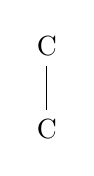
\begin{tikzpicture}[grow'=up]
		\Tree [.C C ] 					
		\end{tikzpicture}												&
		
		
		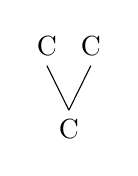
\begin{tikzpicture}[grow'=up]
		\Tree  [.C C C ];
		\end{tikzpicture}			
		&
		
		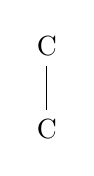
\begin{tikzpicture}[grow'=up]
		\Tree  [.C C ]
		\end{tikzpicture}
		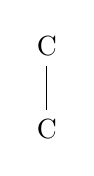
\begin{tikzpicture}[grow'=up]
		\Tree  [.C C ]
		\end{tikzpicture}		
		
	\end{tabularx}
	
	\caption{Autosegmental representation of geminates}
	 \label{fig:Autosegmental representation of geminates} 

\end{figure}

\figref{fig:Autosegmental representation of geminates} shows the autosegmental representations of singletons, lexical geminates and morphological geminates (for similar analyses see, for example,  \citealt[413]{Kenstowicz.1994}, \citealt[26 f.]{Gussmann.2002} and \citealt[62]{Ridouane.2010}). The upper tier shows the skeletal tier and the lower the segmental. While singletons only take one slot at both levels, lexical geminates occupy one slot at the segmental tier and two slots on the skeletal tier. The two prosodic slots account for the long duration of the geminate, as well as for its ambisyllabicity. The single slot on the segmental tier represents the geminate's inalteribility and integrity. Since morphological geminates differ from lexical geminates in terms of their integrity and inalteribility, they take two slots on both tiers. This also mirrors their derivational nature, which naturally entails that a morphological geminate is made of two concatenated identical segments.


Differently from the autosegmental approach, the moraic approach does not entail a segmental prosodic tier on which the geminate is represented as having two slots. Instead, the root-node is directly connected to a higher prosodic structure, i.e. the mora, which represents a segment's underlying weight. \figref{fig:Moraic representation of geminates} shows the moraic representation of singletons, lexical and morphological geminates. While lexical geminates are underlyingly heavy, i.e. moraic, singletons are light, i.e. not moraic. Morphological geminates are represented as two identical singletons. These singletons are regarded as independent from each other and are therefore not underlyingly moraic  (for similar analyses see, for example,  \citealt[14]{Ham.2001}, \citealt[17]{Davis.2014} and \citealt{Davis.2017}).


\begin{figure} [h]
	\centering
	
	
	\begin{tabularx}{.8\linewidth}{YYY}
		
		&		lexical			 & 		 morphological \\
		
		singleton	&			  geminate	 & 			  geminate\\		
		\\
		\begin{tikzpicture}
		\Tree [.C  ] 					
		\end{tikzpicture}												&
		
		
		\begin{tikzpicture}[grow'=up]
		\Tree  [.C $\mu$ ]
		\end{tikzpicture}			
		&
		
		\begin{tikzpicture}[grow'=up]
		\Tree  [.C ]
		\end{tikzpicture}
		\begin{tikzpicture}[grow'=up]
		\Tree  [.C  ]
		\end{tikzpicture}		
		
	\end{tabularx}
	
	\caption{Moraic representation of geminates} 
	\label{fig:Moraic representation of geminates}
\end{figure}


Comparing the segmental and the moraic approach, it is striking that while the representation of lexical geminates differs between the two approaches, morphological geminates are represented as two underlying segments in both analyses.
In this book I will adopt this view and assume that the underlying representation of morphological geminates consists of two segments. In word-medial position one of the segments is in coda position, the other forms the onset of the following syllable. 


While the underlying representation of morphological geminates as two distinct segments seems undisputed, it is yet unclear how these two identical segments are realized at the phonetic level. As described in \sectref{Morphological Gemination}, only few studies on morphological gemination exist. Most of these studies do not systematically investigate important lexical factors which might influence the realization of morphological geminates (e.g. morphological category and decomposability). These factors are, however, important to look at since their role in gemination can provide us with important insights about the morpho-phonological, as well as as the morpho-phonetic interface (see chapter \ref{Theory} for a thorough discussion). 
In this book, I will empirically investigate morphological gemination with English affixes. I will systematically test which factors influence the phonetic realization of morphological geminates with \prefix{un}, locative \prefix{in}, negative \prefix{in}, \prefix{dis} and \suffix{ly}, and thereby contribute new insights to the understanding of morphological geminates and morpho-phonological theory.


\section{Gemination in English} \label{Gemination in English}

The theoretical literature only sparsely discusses morphological gemination in English. The phenomenon is mostly mentioned implicitly and rarely discussed in more than one sentence.  Assumptions about gemination in English can, however, be gleaned from some  theoretically oriented studies and from secondary sources such as handbooks, textbooks or pronunciation dictionaries. Additionally it is possible to deduce predictions about gemination behavior of English affixes from morpho-phonological theories and psycholinguistic approaches of morphological processing. In this section, I will restrict my discussion of English gemination to explicit mentions in the literature, as well as previous empirical studies on the topic. While I will concentrate on gemination with the affixes under investigation, I will also review general statements about gemination in English, i.e. I will take a look at mechanisms which are generally assumed to govern gemination in English, including gemination in compounds and phrases.
In chapter \ref{Theory}, I will then turn to prominent formal linguistic and psycholinguistic approaches, as well as prominent theories of speech production. I will discuss those approaches in detail, and deduce clear predictions about the gemination behavior of the affixes \prefix{un}, \prefix{in}, \prefix{dis} and \suffix{ly}.\footnote{An earlier version of this section has been published in \cite{BenHedia.2017}.}
\label{assumptions}
 

\subsection{Assumptions } \label{assumption gem English}
% I will first take a look at how pronunciation dictionaries treat morphological geminates in \prefix{un}, \prefix{in}, \prefix{dis} and \suffix{ly}-affixed words. I will then move forwards to explicit mentions of gemination with these affixes in the phonological and morphological literature. I will end this review with some general statements found in the 
 % Prinunciation dictionaries
I will start this review by looking at how pronunciation dictionaries (e.g. \citealt{Kenyon.1953, Roach.2011, Wells.2008}) treat morphological geminates in \prefix{un}, \prefix{in}, \prefix{dis} and \hbox{-}\textit{ly}-affixed words.  There is a systematic difference between the representations of the prefix \prefix{in} and the prefix \prefix{un} in the dictionaries. If the prefix \prefix{un} is attached to a base starting in /n/, the word is transcribed with a long nasal (i.e. with [nː]). In contrast, if the prefix \prefix{in} attaches to a base starting with /n/, the transcription only shows a short /n/ (i.e. [n]). The only exception is the word \textit{innavigable} in \citet{Roach.2011}, where the word is transcribed with two [n]s. It is unclear what distinguishes this word from the other \prefix{in}prefixed words. 
  With \prefix{in}, there is the complication that the prefix has three additional variants that may or may not involve gemination: \textit{im-}, \textit{ir-} and \textit{il-}, as in \textit{immobile}, \textit{irresponsible} and \textit{illegal}, respectively. In the dictionaries one consistently finds a short consonant in these cases, too. That is, all allomorphs of \prefix{in} are taken to behave in the same way with regard to degemination.
  
 For the prefix \prefix{dis}, variation is found in \cite{Roach.2011}. While some types are transcribed with two fricatives (e.g. \textit{dissatisfy, dissimulation}), most types are transcribed with only one /s/ (e.g. \textit{dissolution, dissemble)}. It is unclear on which bases it is decided whether a type is transcribed as featuring one or two consonants. There even is variation among types of the same root. While \textit{dissimulation} is transcribed with two /s/, \textit{dissimulate} is transcribed with only one. Interestingly, in \cite{Roach.2011}  a long fricative (i.e. [s\textlengthmark]) is never assigned to \prefix{dis}prefixed words. This suggests that, according to \cite{Roach.2011}, morphological geminates are realized differently in \prefix{dis}prefixed words than in \prefix{un}prefixed words. In contrast to doubles with \prefix{dis}, doubles with \prefix{un} are transcribed with a long nasal (i.e. [n\textlengthmark])  instead of with two (i.e. [nn]).
 Differently from in \cite{Roach.2011}, in \cite{Wells.2008} there is no variation found for \textit{dis}-prefixed words. All types are transcribed with only one /s/, suggesting that \prefix{dis} always degeminates. 
  
  For \suffix{ly}-suffixed words, one finds an interesting note on gemination in \cite{Wells.2008}, stating that ``after a stem ending in l, one l is usually lost'' (451). \cite{Wells.2008} thus suggests that \hbox{-}\textit{ly}-suffixed words degeminate.
 % shall I look up some words in the dictionaries for ly?
 
 Pronunciation dictionaries, which generally consider citation forms unaffected by context-specific or situation-specific influences, thus suggest gemination for \prefix{un} and degemination for \prefix{in} and \suffix{ly}. For \prefix{dis} the dictionaries do not agree. While one dictionary states that the prefix degeminates in all cases (\citealt{Wells.2008}), another one predicts cases in which at least some of the morphological geminates are pronounced as two consonants (\citealt{Roach.2011}).
 
 
Turning to the pertinent phonological or morphological literature, a similar picture emerges for the prefixes \prefix{un} and \prefix{in}, which are the most prominent, and hence the most discussed, examples for morphological gemination in English. \citet[141]{Wijk.1966}, \citet[255]{OConnor.1973}, \citet[18]{Mohanan.1986}, \citet[119 ff]{Borowsky.1986}, \citet[111]{Catford.1988}, \citet[106]{Kreidler.1989}, \citet[251]{Ladefoged.1993}, \citet[18]{Harris.1994}, \citet[22]{Spencer.1996}, \citet[1055 f.]{CohenGoldberg.2013}, and \citet{Cruttenden.2014} all agree that \prefix{un} geminates. Remarks on \prefix{in} are less frequent, and often only refer to isolated pertinent words, but those authors who mention the issue of double nasals with \prefix{in} all agree that \prefix{in} degeminates (\citealt[251]{Ladefoged.1993}; \citealt[18]{Mohanan.1986}; \citealt[18 ff]{Harris.1994}; \citealt[248]{Cruttenden.2014}; \citealt[1055 f]{CohenGoldberg.2013}).

The affixes \prefix{dis} and \suffix{ly} are far less frequently discussed in the literature. 
The adverbial suffix \suffix{ly} is only mentioned implicitly in some of the literature mentioned above. In those works, derivatives with \suffix{ly} are used as examples of words which geminate (cf. \citealt[141]{Wijk.1966}; \citealt[23]{Harris.1994}; \citealt[22]{Spencer.1996}). In contrast, \citet[82]{Bauer.2001}, \citet[353]{Giegerich.2012} and \citet[169]{Bauer.2013} claim variation with \suffix{ly}. Some \suffix{ly}-suffixed words are believed to geminate (e.g. \textit{stalely} and \textit{vilely}) and some are believed to degeminate (e.g. \textit{fully} and \textit{really}). For \suffix{ly}-affixed words in which the suffix occurs after the suffix \suffix{al}, degemination is claimed (e.g.  \textit{federally}, \textit{globally}, \textit{spiritually}). \citet[169]{Bauer.2013} furthermore state that degemination is variable with yet some other words (e.g. \textit{dully} and \textit{wholly}). 
For the prefix \prefix{dis}, there is no discussion which explicitly mentions the gemination behavior of the prefix. Assumptions about \prefix{dis} can therefore only be gleaned from general statements about gemination in English, as well as from dictionary entries, which are, as described above, contradictory. 

After looking at specific mentions of the affixes in the literature, let us now turn to more general thoughts on gemination in English, i.e. the general mechanisms believed to govern gemination in English. 
Most of the discussed literature claims that the affix involved is decisive for the phonetic realization of a double consonant. They assume gemination to be a categorical, i.e. not a gradient, phenomenon. The majority of approaches accounts for the alleged difference in gemination behavior between affixes by positing two different kinds of morphological boundary. \citet[18]{Mohanan.1986} and \citet[119 ff]{Borowsky.1986}, in the framework of Kiparskian lexical phonology (\citealt{Kiparsky.1982} et seq.), for example, assign \prefix{in} to level 1 and \prefix{un} to level 2. In this theory, level 1 affixes have weak morphological boundaries which go along with greater phonological integration with their base, including assimilation and degemination. Level 2 affixes, in contrast, form strong boundaries with their base and are phonologically less integrated. Hence, gemination is expected for level 2 affixes. Similar in spirit is \citeauthor{Harris.1994}' (1994) account, in which the author distinguishes between root affixation (for \prefix{in}) and word affixation (for \prefix{un} and \suffix{ly}). In root-affixation, generally one phoneme is deleted when two identical segments immediately follow each other. 
\cite{CohenGoldberg.2013} attributes the alleged difference in gemination between \prefix{in} and \prefix{un} to their difference in  productivity: the less productive prefix \prefix{in} degeminates, while the more productive \prefix{un} geminates. 
\citet[354]{Giegerich.2012} proposes that gemination depends on the phonological word status of the derivative. The phonological word status, similar to productivity, mirrors morphological boundary strength. Only derivatives with weak morphological boundaries form prosodic words (see \sectref{prosodic word} for discussion). According to \cite{Giegerich.2012}, geminates only occur across prosodic word boundaries, which is why most \suffix{ly}-derivatives, which form a prosodic word with their base, degeminate.

\citet[169]{Bauer.2013} describe gemination to be less predictable, i.e.  to be not solely  predictable by the affix involved. They, in contrast to the approaches discussed above, assume variation within the gemination pattern of one affix. Furthermore, the authors point at possible variables, other than the affix, which could have an effect on gemination (e.g. speech tempo and the speaker). Similarly \citet[191, 288]{Giegerich.1992} notes the effect of speech mode by stating that geminates are usually simplified in connected speech.
 
 
One can summarize that most of the theoretical literature, as well as pronunciation dictionaries, assume gemination to be affix-dependent. Different boundary strengths between affixes are assumed to cause differences in gemination. While the nature of the boundary deviates between different approaches, the main idea is that stronger boundaries lead to gemination and weaker boundaries lead to reduction, i.e. degemination. Only few sources assume that factors other than the affix involved influence gemination, and that variation in gemination can be found in words compromising the same affix.  In chapter \ref{Theory}, I will return to the different ideas proposed and discuss them in more detail. 

Summarizing the affix-specific predictions, one can state that for \prefix{un} and \prefix{in}, pronunciation dictionaries, as well as the majority of the theoretical literature, agree that the former geminates, while the latter degeminates. Less is said about \prefix{dis} and \suffix{ly}. For \prefix{dis}, dictionaries make contradicting assumptions and the theoretical literature is silent about its gemination behavior. For \suffix{ly}, one also finds contradicting predictions. While \cite{Wells.2008} states degemination, the majority of the theoretical literature claims gemination with \suffix{ly}. Some of the literature predicts variation. 

\subsection{Previous empirical work}\label{previous empirical work}

Apart from \cite{BenHedia.2017}, which is given in chapter \ref{Corpus Studies}, there are five studies on gemination in English: \cite{Delattre.}, \cite{ Kaye.2005}, \cite{Oh.2012}, \cite{Oh.2013}   and \cite{Kotzor.2016}.   % Delattre
The first study by \cite{Delattre.} looked at word-boundary geminates. Delattre compared the duration of double consonants at word boundaries (such as the double nasal  in the sentence "\textit{I've seen Nelly}") with word-final singletons (such as the nasal in "\textit{I've seen Elly}") and word-initial singletons (such as the nasal in "\textit{We see Nelly}"). He investigated three different segments: /n/, /l/ and /s/. For all three he found that word-boundary geminates are longer than singletons. The nasal showed the highest degree of gemination (singleton-geminate ratio: 1:1.5). The fricative and the lateral had a singleton-geminate ratio of 1:1.3. Interestingly, the duration of the preceding segment did not vary depending on the number of consonants. In other words, gemination did not affect preceding vowel duration.

Even though this study shows that morphological gemination in English may lead to longer durations, it can only be regarded as a first clue to understand gemination in English. Since Delattre solely looked at word-boundary geminates, i.e. not at other types of morphological boundary, it remains unclear which role morphology, and consequently different boundary strengths, actually plays in the realization of geminates. Furthermore, there are major methodological issues. Delattre's results are based on only a few types and it is thus unclear which role type-specific effects might have played. The study did furthermore not account for possibly intervening factors such as, for example, speech rate. Another drawback of the study is its lack of appropriate statistics. Taking all of these drawbacks into account one can nevertheless assume that morphological gemination at word boundaries in English does, at least in some cases, lead to gemination.


\citet{Kaye.2005} and \citet{Oh.2012} both empirically investigated gemination with the two English prefixes \prefix{un} and \prefix{in}. In both studies the gemination of \prefix{in}prefixed words was investigated by looking at words that featured the allomorph \textit{im-}. The reason for this is that there are very few \prefix{in}prefixed words with a base starting in /n/ (such as \textit{innumerous}), i.e. there are not enough different types to empirically investigate gemination with \prefix{in} (see \sectref{theory:in} for further discussion). 


\cite{Kaye.2005} investigated  only two \prefix{un}prefixed types (\textit{unknown, unnamed}) and one \prefix{in} prefixed type (\textit{immature}). In an elicitation task, ten speakers produced these words, as well as the words’ bases in isolation. Kaye then compared the durations of the nasals in the different words. The results indicate that both prefixes geminate. The [n] in \textit{unknown} is longer than the [n] in \textit{known},  the [n] in \textit{unnamed} is longer than the [n] in \textit{named} and the [m] in \textit{immature} is longer than the [m] in \textit{mature}. Kaye notes, however, that whether an \prefix{in}prefixed word geminates or not depends  on the individual speaker. Not all speakers produced the prefixed words with a longer nasal than the base. However, since Kaye did not apply any statistical analyses (beyond computing averages) and only investigated a very limited number of types, the results are somewhat inconclusive. What we can see, however, is that Kaye's empirical data go against the claim that \prefix{in} always degeminates.


\cite{Oh.2012} also investigated gemination with \prefix{un} and \prefix{in}, as well as gemination at word boundaries  (e.g. \textit{dim morning, one nail}). With regard to gemination with \prefix{in} and \prefix{un}, they compared the duration of morphological geminates with the duration of assumed phonological singletons in words starting with similar phonemic strings. The authors investigated 16 different words which contained two consonants in the orthographic representation.  The items were categorized  by Korean speakers (i.e. speakers of a language that has phonological geminates) who rated the duration of the nasals as either single or double, based on an English native speaker’s pronunciation of these words. The words \textit{immovable, immoral, immemorial, immeasured, unnoticed, unnamed, unnerve, unnail} were categorized as containing a double nasal, while \textit{ammonia, immensely, immunity, immigrational, annex, innate, annoyed, innerve} were categorized as words containing a single nasal. 
Additionally, Oh and Redford included word-boundary geminates (e.g. \textit{dim morning, one nail}) in their data set to investigate potential differences between word-internal and word-boundary geminates. All items were put into carrier sentences and read by eight participants in two different conditions (normal speech vs. careful speech). 

With regard to word-internal geminates the analyses showed that the items rated by Korean speakers as having double nasals were longer in duration than items rated as having single nasals. This indicates that at least some words with the prefix \prefix{in} show gemination.
However, there is variation in the gemination pattern of \prefix{in} found by \cite{Oh.2012}: the set of words with singletons mainly contains words that are morphologically simplex, but some words are not simplex. The word \textit{immigrational}, for example, is prefixed (compare \textit{migration}, \textit{immigration}), which in turn means that in this word, \prefix{in} degeminates, while in the other prefixed words it geminates. Note also that \prefix{in} in the word \textit{immigrational} (like, arguably, \textit{innate} `existing in a person [...] from birth', \textit{OED online}\nocite{OED.2013}, s.v. `innate, adj.'), has a locative meaning. Incidentally, both words in which we find \prefix{in} as a locative prefix ended up in the set of words that do not geminate, while the words with negative \prefix{in} showed gemination. This might hint at a systematic difference between locative and negative \prefix{in}, an issue that is never discussed in the theoretical literature.

The study also reveals general differences between the two prefixes \prefix{un} and \prefix{in}. \cite{Oh.2012} found a difference in absolute nasal duration between the two prefixes. The nasal in \prefix{in}prefixed words is significantly shorter than the nasal in \prefix{un}prefixed words. This difference is more prominent in careful speech than in normal speech. The durational difference between the prefixes vanishes, however, in relative duration. Relative duration refers to the nasal duration relative to the duration of the preceding vowel. This means that not only nasal duration differs between the two prefixes but that there is also a difference in preceding vowel duration. The prefix \prefix{un} features a longer vowel than the prefix \prefix{in}.  In other words, \prefix{un} is generally longer than \prefix{in}. In addition to prefix duration, \cite{Oh.2012}
also found non-durational differences between \prefix{un} and \prefix{in}. In careful speech, speakers sometimes inserted a pause between the two nasals of \prefix{un}prefixed words, whereas a pause was never inserted in \prefix{in}prefixed words. The authors interpret the inserted pause as a boundary cue.

Turning to word-boundary geminates,  results revealed that there was no durational difference in absolute duration between word-internal and word-boundary geminates. There was, however, a difference between the two types of geminates in relative duration. Word-boundary geminates were shorter than word-internal geminates, and as long as singletons in relative duration. In other words, while geminates in \prefix{un} and \prefix{in}prefixed words are longer than singletons in absolute and relative duration, word-boundary geminates are only longer than singletons in absolute duration.


Oh and Redford interpret their results as evidence that word-boundary geminates are represented differently than word-internal geminates, i.e. that gemination is influenced by boundary strength.  Furthermore, they argue that the prefix \prefix{un} might be represented differently than the prefix \prefix{in}. They base their argument on the finding that, even though there does not seem to be a systematic difference in the gemination behavior of the two prefixes, the two prefixes display differences in their overall duration, as well as differences with regard to non-durational boundary cues. \cite{Oh.2012} venture the idea that different affix representations emerge from differences in boundary strength (cf. \citealt{Kiparsky.1982,Mohanan.1986}, see \sectref{LexPhon} for discussion), or from differences in productivity and segmentability (cf. \citealt{Hay.2003}, see \sectref{Morphological Gemination: Implications for Psycholinguistic Theories of Morphological Processing} for discussion). Since the prefix \prefix{un} has a stronger boundary than \prefix{in}, and since it is more productive and segmentable, there is less reduction with \prefix{un} than with \prefix{in}, i.e. it is longer and features boundary cues.


To investigate the relation of different morphological boundaries and gemination further, in a follow-up study \cite{Oh.2013} investigated whether there is a difference between geminates at compound-internal boundaries (e.g. \textit{homemade}) and geminates at word boundaries (e.g. \textit{room maid}). The comparison of geminate durations and the duration of singletons at word boundaries (e.g. \textit{dough made}) showed that both types of geminates are longer than singletons. A significant difference between compound-internal and word-boundary geminates is only found in careful speech, and only in absolute consonant duration. In accordance with the idea that word-boundary geminates have a stronger morphological boundary than compound-internal geminates,  in careful speech word-boundary geminates are longer. In normal speech the difference vanishes. For relative duration, there never is a difference between compound-internal and word-boundary geminates. \cite{Oh.2013} interprets the results as there not being a difference in the realization of compound-internal and word-boundary geminates in English. 


Thus, while in \cite{Oh.2012} there might be some indication for effects of boundary strength on gemination (difference between word-internal and word-boundary geminates in relative duration), we do not find these effects in \cite{Oh.2013}. There are various possible explanations. 
It might for example be that only certain boundary differences lead to differences in gemination. This explanation ties in with the results on morphological gemination in German, Tashlhiyt Berber and Maltese discussed in \sectref{Morphological Gemination}. These studies also showed that, while gemination differed between some types of boundaries, it did not between others. 
Another explanation for the deviating results might be related to the studies' methodologies.  
Both studies only investigated a very low number of types, which prohibited to test the influence of type-specific factors on duration. Furthermore, there might be other intervening factors such as, for example, speech rate and speaker, which influence duration, and which were not systematically  taken into account. 
With regard to methodology another crucial aspect must be considered when interpreting the results.
The studies show differences in effects depending on the acoustic correlate used as the measure of gemination. Effects are different for absolute and relative duration. There are also differences depending on speech condition, i.e. careful vs. normal speech. 
Especially the different outcomes depending on speech condition suggest that factors related to the experimental set-up influence results of durational studies to a great degree. It is yet unclear how to interpret the relation between the different outcomes and the different conditions.
To shed light on the matter, it is necessary to conduct further studies which systematically compare experimental data with conversational speech, and which control for intervening factors in a systematic way. More advanced statistics, which are able to tease apart different effects, are necessary to explain which factors cause which durational differences, and whether it is indeed boundary strength which leads to differences in gemination between different words and constructions.



The most recent study on gemination in English looked at gemination in suffixation and compounding. Using a reading experiment, \cite{Kotzor.2016} investigated the two suffixes \suffix{ly} and \suffix{ness}, as well as compounds with sonorant ([l] and [n]) and stop geminates ([p], [t] and [k]). With respect to the suffixed data, they compared the double consonant with the singleton in the pertinent base word to which the suffix \textit{-er} was added. Hence, the double consonants in \suffix{ness}- and \suffix{ly}-suffixed words (e.g. /nn/  and /ll/ in \textit{coolly} and \textit{meanness}) were compared to the pertinent singletons in \textit{-er}-suffixed words (e.g. /n/ and /l/ in \textit{meaner} and \textit{cooler}). The doubles in compounds (e.g. /nn/ in \textit{pine nut}) were compared to singletons in similar compound words (e.g. /n/ in \textit{pineapple}). 
The results reveal that both types of geminates, i.e. suffixational and compound geminates, are longer than the pertinent singletons. There was no effect of the geminate on the preceding vowel duration, neither for the suffixes, nor for the compounds. Thus, \cite{Kotzor.2016} did not find a significant difference between the gemination of suffixes and compounds. 

Unfortunately, \cite{Kotzor.2016} do not provide a separate analysis for each of the two suffixes. In other words, their analysis does not provide the possibility to state whether the suffixes \suffix{ness} and \suffix{ly} behave differently with regard to their gemination behavior. This can be regarded as a major drawback of the study since, as described in \sectref{assumptions}, it is commonly assumed that gemination is affix-dependent. From a theoretical point of view there is good reason to assume that the two suffixes \suffix{ly} and \textit{-ness} do not behave identically. 
This idea is further supported by the fact that geminate duration varies among different types of consonants (cf. \sectref{what is gemination}). The lateral in \suffix{ly}-words is expected to inherently show different durations than the nasal in \textit{-ness}-words. Furthermore, there might be structural differences between the two affixes, such as their segmentability and boundary strength, which might lead to different behavior regarding gemination. 
An additional problem with the study is the limited number of types investigated. For each affix only six types with a morphological geminate were included, making it impossible to investigate type-specific effects such as word-form frequency or a word's individual decomposability. Thus, even though the study provides some evidence for the gemination of \suffix{ly} and \suffix{ness}, one must be cautious to interpret the results. Further research on the individual suffixes incorporating a greater number of different types is necessary to make reliable statements about their gemination behavior.


To summarize, previous research on gemination in English leaves us with a number of unsolved problems. First, there is only little empirical evidence available and the few studies which do exist differ significantly in their methodology and the constructions they investigated. Hence, the facts essentially are unclear. Only three studies looked at affixational gemination in English, i.e. the phenomenon under investigation in this book (\citealt{Kaye.2005, Oh.2012, Kotzor.2016}). Two of these studies (\citealt{Kaye.2005, Oh.2012}) call the assumption that \prefix{in} degeminates into question, and hence demonstrate the need for further testing of widely-held beliefs about gemination in English. 

Second, existing empirical studies are rather limited in their data sets and consider only words spoken under experimental conditions, i.e. in isolation or in carrier sentences. What is lacking is data from natural speech. As pointed out in the literature (e.g. \citealt{Giegerich.1992, Bauer.2013}), and as evidenced by \cite{Oh.2012} and \cite{Oh.2013}, the mode of speech might significantly influence the realization of morphological geminates. Therefore, it is necessary to investigate the phenomenon in various conditions, making it possible to compare natural speech with experimental data. This will allow us to find out which factors influence gemination on which level.

Third, existing studies have not simultaneously considered different influences which might affect gemination, but rather concentrated on one specific aspect, i.e. they neglected other possibly intervening factors. None of the studies described above has looked at word-specific factors, such as word-form frequency or a word's individual decomposability. Even though, as shown in \sectref {assumptions}, most claims about gemination are based on morphological categories, morphological factors were only considered sparsely in previous research. While most studies pointed out that different morphological categories, such as different affixes or derivatives with varying morphological boundary strength, might differ in their gemination behavior, their methodology was insufficient to shed light on the matter. 
The studies comparing \prefix{un} and \prefix{in}, for example, just assumed a categorical difference in boundary strength between the two affixes. This assumption needs to be empirically investigated. Furthermore, the investigation of \prefix{in} did not consider that there are two different \prefix{in}prefixes, i.e. locative and negative, and that there are potential differences between them. The study on the two suffixes \suffix{ly} and \textit{-ness} did not differentiate between the two suffixes at all, just assuming a similar behavior of both of them. 

To conclude, previous research hinted at some interesting effects, such as the gemination of affixes which are assumed to degeminate, and differences in gemination depending on the type of morphological boundary involved. However, due to mainly methodological reasons further research is needed to clarify facts.


%  
\chapter{The Affixes under investigation}{\label{affixes}}


In this chapter I will describe the five affixes \prefix{un}, negative \prefix{in}, locative \prefix{in}, \prefix{dis} and \suffix{ly} using the relevant morphological and phonological literature. I will discuss their phonological behavior, as well as important morphological, semantic and lexical properties, and compare them with regard to these factors.

Before discussing the affixes, I will give a brief overview of the factors which lead to their inclusion in this study.
The prefixes \prefix{un} and \prefix{in} were included because of two reasons.
First, they are the most prominent examples of \isi{gemination}/\isi{degemination} given in the literature (see discussion in \sectref{assumptions}).  Second, they are investigated empirically in two previous studies, i.e. a comparison to previous results is possible. 
To investigate an additional prefix, and to also take a look at \isi{gemination} in suffixes, the affixes \prefix{dis} and \suffix{ly}  were added to the data set. The choice to include these two affixes was on the one hand due to their comparatively high type \isi{frequency}, which allows for testing type-specific effects on \isi{gemination}, and  on the other due to their phonological and morphological make-up.
The five affixes partly overlap in their characteristics, such as their semantics, their prosodic make-up and their \isi{segmentability}. Importantly, they also show some major differences in their features. This combination of similarities and differences between the affixes makes it possible to test various factors which potentially affect \isi{gemination} across affixes.

In the following, I will describe the formal and structural characteristics of each affix, lay out their phonological and prosodic behavior, as well as discuss their semantics. Since the literature is often not very specific, or even contradictory when discussing certain aspects of \isi{affixation} (e.g. \isi{stress} pattern or \isi{productivity}), it is often not possible to give a clear-cut description of a certain affix and its behavior. I will remain neutral regarding most of the controversial issues but lay out the different possibilities, as found in the literature.  

After looking at each affix in isolation, I will compare the five affixes with each other. It is of prime importance to look at the differences between the affixes, since these differences lead, according to the theories discussed, to different predictions for their \isi{gemination} behavior. I will pay special attention to \isi{boundary strength} as it is one of the most important factors for predicting \isi{gemination}.  
At the end of this section, I will provide some insightful figures regarding the scope of the phenomenon across affixes. In other words, I will lay out how many types with a \isi{morphological geminate} exist for each affix.

\section{Description of the affixes}

\subsubsection{The prefix \prefix{un}} {\label{description un}}

The affix \prefix{un} is a native prefix which takes native and non-native bases. According to \citet[ 355, 361, 371 ff]{Bauer.2013}, its bases can be verbs, nouns and adjectives. The prefix rarely changes the category of its base and does not take bound roots. It is one of the most productive prefixes in English and has a clearly negative meaning, which varies slightly depending on the base it attaches to. On verbs its meaning is reversive (e.g. \textit{screw} vs. \textit{unscrew}) and sometimes privative (e.g. \textit{dress} vs. \textit{undress}), on adjectives its meaning is contrary or contradicting (e.g. \textit{cool} vs. \textit{uncool}), and on nouns it mostly is privative (e.g. \textit{faith} vs. \textit{unfaith}).
In general, the meaning of \prefix{un}derivatives is very transparent. Only few forms exist in which one cannot deduce a derivative's meaning by adding the negative meaning of \prefix{un} to that of its base (e.g. \textit{unorthodox}).

Turning to the prefix's phonological attributes, \prefix{un} shows what can be called `optional assimilation'. This assimilation affects \prefix{un}derivatives with a base starting in a bilabial (e.g. \textit{unplugged, unbreakable, unmarried}) and \prefix{un}derivatives with a base starting in a velar plosive (e.g. \textit{ungrateful, uncool}).
Before bilabials the prefix-final nasal sometimes is realized as [m]. Before velar plosives the prefixal nasal sometimes is velarized, i.e. realized as [ŋ] (cf. \citealt[5 f]{Hanote.2010}; \citealt[180]{Bauer.2013}; \citealt[125]{Okada.2013}). 
This optional assimilation is not mirrored in \isi{orthography} and, according to \citet[125]{Okada.2013}, is purely phonetic, i.e. not phonological, in nature. \citet[87 f]{Stockwell.2001} explain the optional assimilation of \prefix{un} by a conflict between `ease of pronunciation' and `transparency'. While the assimilation of the nasal makes pronunciation easier, the transparent nature of the prefix blocks the total assimilation of the prefix.
Except for one study (\citealt{Hanote.2010}), there is, according to my knowledge, no empirical work on the assimilation of English \prefix{un}. \cite{Hanote.2010} found no systematic pattern with regard to assimilation with \prefix{un}. However, since the authors restricted their study on dictionary data it is questionable how generalizable their results are.  
As \citet[138]{Raffelsiefen.1999}, for example, proposes, assimilation with \prefix{un} might be sensitive to register.  According to her,  assimilation is most likely to occur in fast, \isi{casual speech}. This would mean that dictionary data is not suited to investigate the matter.
To conclude, \prefix{un} sometimes assimilates but the pattern of its assimilation is yet unclear.




Before discussing the \isi{stress} status of \prefix{un}, a general note on prefix \isi{stress} is in order. The \isi{stress} of prefixes is not well researched and observations are mostly anecdotal, i.e. rely on individuals' intuitions rather than on empirical studies. Furthermore, as evidenced in \cite{Videau.2015}, \isi{prefixal stress} depends on various factors, such as \isi{semantic transparency}, syntactic context and extra-linguistic context. It is yet unclear how these factors interact, i.e. it is unclear how exactly they influence \isi{stress} with prefixes.
Even when leaving contextual influences aside, i.e. when concentrating on lexical \isi{stress} in isolated words, it is quite difficult to determine the \isi{stress} pattern of prefixed words. 

The determination of \isi{stress} for monosyllabic prefixes, such as \prefix{un}, \prefix{in} and \prefix{dis}, is of special difficulty. When followed by an unstressed syllable they are, due to prosodic constraints, usually taken to be \isi{stressed}. Matters are, however, more complicated when the prefix is followed by a \isi{stressed} syllable. In those cases it is very challenging to determine the relative prominence relations between the prefix and the base-initial syllable, i.e. it is very hard to determine whether the prefix is \isi{stressed} or not. 
While it is generally assumed that prefixes can bear \isi{stress}, it is unclear how \isi{stress} patterns in those cases. In other words, it is unclear whether the prefix is unstressed, whether it bears primary \isi{stress} or whether it bears secondary \isi{stress}. As discussed in \citet[126]{Okada.2013} for \prefix{un}, \prefix{in} and \textit{non-}, there is variation within prefixes, and this variation ``leads linguists to different descriptions''. 
To summarize, due to difficulties in determining \isi{stress} and the not well researched variation in prefix \isi{stress}, the descriptions of \isi{prefixal stress} deviate between sources for the prefixes \prefix{un}, \prefix{in} and \prefix{dis}. %The \isi{stress} pattern of the prefixes is unclear.


The available descriptions of \isi{stress} with \prefix{un} reflect the problems just pointed out. While \citet[4]{Allen.1978} notes that the prefix never bears \isi{stress}, other sources such as \citet[464 f]{Jespersen.1965} and \citet[126]{Okada.2013} state that \prefix{un} is a stress-preserving prefix that may carry \isi{stress}. Similarly in \cite{Wells.2008} \prefix{un} can be \isi{stressed}. Except for \cite{Allen.1978}, all sources agree that \prefix{un} is \isi{stressed} if the base-initial syllable of the pertinent derivative is unstressed (e.g. \textit{ˌunconˈventional}\footnote{Throughout this book I will use ˈ to mark primary \isi{stressed} syllables and ˌ to mark secondary \isi{stressed} syllables.}).
Assumptions deviate for those cases in which the first syllable of the derivative's base is \isi{stressed} (e.g. \textit{unˈjust}). \citet[464 f]{Jespersen.1965} notes for these cases that, while in some of the most common \prefix{un}derivatives the prefix is unstressed (e.g. \textit{unˈcommon, unˈhappy}), in most cases the prefix is \isi{stressed} (e.g. \textit{ˈunˈaided, ˈunˈjust}). 
In \citet[808]{Wells.2008} it is noted that while generally the prefix may be either \isi{stressed} or unstressed in those cases, verbs always have a \isi{stressed} prefix (e.g. \textit{ˌunˈcoil}). Furthermore, it is noted that \prefix{un} ``is unstressed particularly where it is not a true prefix (\textit{unˈwieldy})'' (808). Wells does not give a definition of true prefixhood though, i.e. this statement is quite unclear. Divided or uncertain usage is annotated for some of the \prefix{un}prefixed words with a \isi{stressed} base-initial syllable (e.g. \textit{\textsubscript{(}ˌ\textsubscript{)}unˈbearable, \textsubscript{(}ˌ\textsubscript{)}unˈleash}). As evidenced in a study by \citet[2 ff]{Hanote.2010}, the assignment of \isi{prefixal stress} with \prefix{un} in \cite{Wells.2008} does not follow any systematic pattern.
On can thus state that the literature does not provide clear, systematic and empirically-based criteria for \isi{stress} in derivatives with a \isi{stressed} base-initial syllable. It therefore remains unclear when \prefix{un} is \isi{stressed} and when it is unstressed. 


One can summarize that \prefix{un} is a very segmentable and very productive prefix. Its meaning is clearly negative and transparent in the vast majority of derivatives. The fact that \prefix{un} only optionally assimilates can be interpreted as a result of its high \isi{segmentability} which blocks total assimilation, and  which hence ensures the prefix's phonological independence from its base. With regard to \isi{stress}, one can state that \prefix{un} can bear \isi{stress} but that the \isi{stress} pattern of the prefix is yet unclear.



\subsubsection{The prefix \prefix{in}} \label{theory:in}

When investigating the prefix \prefix{in}, one must acknowledge the existence of two different \prefix{in}prefixes in English: negative \prefix{in} and locative \prefix{in}. While the existence of negative \prefix{in} is uncontroversial, the idea of locative \prefix{in} may not be as straightforward. The reason is that locative \prefix{in} often occurs in derivatives with bound roots, such as \textit{inject} or \textit{infuse}. In these words the discrete meaning of \prefix{in}, as well as the discrete meaning of the base, is often unclear. This might lead to the view that locative \textit{in-} is not a prefix but some sort of unit below the word level with  no clear semantic content. This view, however, neglects that locative \prefix{in} does indeed have a stable meaning.  

Let us take the standard methodological approach to morphological categories according to which an affix should have an identifiable, stable meaning across different words (cf., for example, \citealt[chapter 5.2.2]{Plag.1999}; \citealt[63 ff]{Stockwell.2001}; \citealt[68]{Schulte.2015}). Under this approach we would consider \prefix{in} a locative prefix in all those words (and only in those) where the word-initial string \prefix{in} can be assigned some locative meaning and where at the same time the remaining string is also attested outside that word with a stable, identifiable meaning.
Implementing this method, we would be able to assign some locative meaning to the string \prefix{in} in words such as \textit{infuse} `to pour in', \textit{implant} `to plant in' and \textit{import} `to bring in' (\textit{OED online} paraphrases). The remaining strings, i.e. the bases, in these words are all attested (either as words or as bound roots) outside these words with sufficiently similar meaning (cf. \textit{transfuse}, \textit{plant}, \textit{export}). This small sample thus shows that, at least in some words, there is a locative prefix \prefix{in}. 


In this study, all words in which the affix and the base carry a stable meaning are considered as morphologically complex.  Since, complex words with both \prefix{in}prefixes exist, i.e. negative and locative \prefix{in}, both types of \prefix{in} are included in the study.  Below I will take a closer look at each type of \prefix{in}.




\subsubsection{Negative \prefix{in} } \label{negative in}

Differently from \prefix{un}, negative \prefix{in} is a non-native (or Latinate) prefix that takes non-native bases. It mostly takes adjectives as its base (e.g. \textit{intolerant, immortal}). Only sometimes nouns are taken as its base (e.g. \textit{inexperience}).  In most cases, negative \prefix{in} does not change the word class of its derivative.  Usually free bases are found with negative \prefix{in} (e.g. \textit{intolerant, impossible}), but in some derivatives bound roots are found (e.g. \textit{inept, innocent}). In these words it is, however, questionable whether \prefix{in} can even be considered a prefix (cf. \citealt[356 f, 611]{Bauer.2013}).

The majority of the literature claims that negative \prefix{in} is not productive (cf. \citealt[1688]{Bauer.2002}). A search of hapax legomena in the Corpus of Contemporary American English (\citealt{Davies.20082014}), as carried out by \citet[361] {Bauer.2013}, reveals however that there is indeed a number of new derivatives with negative \textit{in}-. Examples are \textit{immedical, inactual, inconservative} and \textit{inextractable}.  One should note, however, that negative \prefix{in} is far less productive than \prefix{un}, which carries similar meaning. Both prefixes denote contrary or contradictory meaning on adjectives.
 Because of these similarities in meaning the prefixes are often treated as rivals. It is often claimed that the existence of a derivative featuring one of the two prefixes blocks the existence of  a derivative with the other. According to this view, the existence of the word *\textit{inhappy}, for example, is blocked by the existence of the word \textit{unhappy} (see, for example,  \citet[467 ff]{Jespersen.1965}, \citet[1688 f]{Bauer.2002} and \citet[377 ff]{Bauer.2013} for discussion).  
As reported by \citet[377]{Bauer.2013}, the idea of rivalry between the two prefixes is, however, invalidated by the existence of derivatives such as \textit{inaccessible} and \textit{unacessible}. There is no noticeable difference in meaning between the two derivatives, and in turn there is no difference in meaning between the two prefixes \prefix{un} and \prefix{in}.
However, while the two prefixes often are identical in meaning, \citet[379]{Bauer.2013}, similar to  \cite{Jespersen.1965} and \cite{Bauer.2002},  note that \prefix{in}derivatives are more often lexicalized than derivatives with \prefix{un}. To summarize, while negative \prefix{in} is very similar to \prefix{un} in its meaning, it does not share its high degree of \isi{productivity} and its consistency with regard to \isi{semantic transparency}.

Turning to the phonological features of negative \prefix{in}, one must mention its obligatory assimilation. Before a bilabial the prefixal nasal becomes /m/. Before a base-initial lateral the nasal becomes /l/, and before an alveolar rhotic it becomes /r/. Examples are \textit{impossible}, \textit{immortal}, \textit{illogical} and \textit{irregular} (cf. \citealt[1687]{Bauer.2002}; \citealt[359]{Bauer.2013}; \citealt[123 f]{Okada.2013}). This assimilation is also mirrored in \isi{orthography}. 

With regard to \isi{stress}, \prefix{in}, similar to \prefix{un}, is generally assumed to be \isi{stressed} when followed by an unstressed syllable (cf. \citealt[473]{Jespersen.1965}; \citealt[381, 384]{Wells.2008};  \citealt[183]{Bauer.2013}; \citealt[126]{Okada.2013}). Examples are \textit{ˌinexˈhaustible, ˌindeˈscribable} and \textit{ˌimmeˈmorial}. In those cases \prefix{in} bears secondary \isi{stress}. There are also some derivatives, such as \textit{ˈimpotent} and \textit{ˈimpious}, in which \prefix{in} is primarily \isi{stressed}. \citet[183]{Bauer.2013} note that while  \isi{stress} with \prefix{in} seems unsystematic in general,  the prefix seems to only bear primary \isi{stress} when the base of the derivative is bound.
In case of a \isi{stressed} base-initial syllable, \prefix{in} is, in contrast to \prefix{un}, generally taken to be unstressed (cf. \citealt{Wells.2008}; \citealt[183]{Bauer.2013}; \citealt[126]{Okada.2013}). 

We can summarize that, while negative \prefix{in} is similar in meaning to \prefix{un}, it is less semantically and phonologically transparent. It is also less productive. Negative \prefix{in} has more bound roots than \prefix{un}, is sometimes semantically opaque, and derivatives are more often lexicalized. The prefix is phonologically more integrated in its base than \prefix{un}. This is indicated by the obligatory assimilation of the prefix. The \isi{stress} pattern of \prefix{in} can also be interpreted as an indicator of its phonological integration. While in some respects the \isi{stress} pattern is similar to the one of \prefix{un}, the prefix, contrary to \prefix{un}, also bears primary \isi{stress} in some cases. Primary \isi{stress} emerges with bound roots and denotes \isi{stress shift}, i.e. in those derivatives the position of primary \isi{stress} has shifted from the base to the prefix. This shows that the boundary between prefix and base is rather weak.\\


\subsubsection{Locative \prefix{in}} \label{locative in}

Locative \prefix{in} differs in interesting respects from negative \prefix{in}. Differently from negative \prefix{in}, the origin of locative \prefix{in} is twofold. This leads to a prominent distinction in the literature. Traditional approaches differentiate between non-native (or Latinate) locative \prefix{in} and native locative \prefix{in}.  While the first one is commonly analyzed as a prefix which takes non-native bases, the second is often analyzed as a locative particle (cf. \citealt[497 ff]{Jespersen.1965}; \citealt[115,163 f]{Marchand.1969}; \citealt[1685]{Bauer.2002}). Examples are given below:

\begin{exe}
	\ex non-native locative \prefix{in}: \hspace{0.7cm} \textit{inject, immigrate, impress}
	\ex native locative \prefix{in}: \hspace{1.4cm} \textit{inborn, inbreed, indoors}
\end{exe}

\cite{Bauer.2013} also make a distinction between the two different cases but regard both types of locative \prefix{in} as prefixes. Since the authors only discuss productive prefixes, and since they consider non-native locative \prefix{in} unproductive,  only native \prefix{in} is discussed in their work. It is said to be a productive prefix that attaches to nouns, adjectives and verbs. It takes native and non-native bases (\citealt[334, 340]{Bauer.2013}).
 
 It is generally assumed that the two types of locative \prefix{in} differ in their type of base, their \isi{productivity} and in the degree of phonological assimilation they display. While the non-native prefix is believed to mostly take non-native bases (see \citealt[499]{Jespersen.1965}), native \prefix{in} also attaches to native bases (see \citealt[334]{Bauer.2013}). While non-native locative \prefix{in} is not productive, the native form is believed to be productive. With regard to phonological assimilation, non-native \prefix{in} undergoes the same obligatory assimilation as negative \prefix{in}, while native locative \prefix{in} is described as only optionally assimilating (see \citealt[499]{Jespersen.1965}; \citealt[335]{Bauer.2013}). The common assumption thus seems to be that non-native locative \prefix{in} is phonologically and semantically less transparent than native locative \prefix{in}. There are, however, no empirical studies investigating whether these criteria mirror the distinction between the two types of locative \prefix{in}. 
 

It is not easy to distinguish between  between native and non-native locative \prefix{in}. This problem is  already discussed in early works such as \citet[499]{Jespersen.1965} and \citet[164]{Marchand.1969}. The semantics of both types of locative \prefix{in} overlap to a high degree. Both prefixes denote a locative meaning, which is formulated as ‘into, in, within; on, upon; towards, against’ in the \textit{OED online}\nocite{OED.2013}. The \textit{OED} further mentions that 

\begin{displayquote}
``[s]ince \prefix{in} prefix 1 [non-native \prefix{in}] and \textit{ in-} prefix 2 [native \prefix{in}] are identical in form, and to a great extent in sense, they come in later use to be felt as one and the same prefix; and it is this resulting prefix which appears in many words of later formation.''
\end{displayquote}

It is thus suggested that, while locative \prefix{in} has two origins, the distinction between the two formerly distinct types of locative \prefix{in} is no longer clear. This is in line with the observation that the criteria used to distinguish native from non-native locative \prefix{in} are rather blurry. 
In this study, I will not explicitly distinguish between the two types of locative \prefix{in}. I will, however, account for differences in \isi{semantic transparency}, phonological make-up and type of base in my studies. I therefore will be able to implicitly differentiate between more \isi{decomposable} and less \isi{decomposable} locative \prefix{in}derivatives, which in turn, according the literature, may mirror the distinction between native and non-native locative \prefix{in}.

With regard to \isi{stress}, the literature is mostly silent about a distinctive \isi{stress} pattern for locative \prefix{in}. Except for \citet[384]{Wells.2008}, who notes that \prefix{in} is ``generally \isi{stressed} only
(i) if meaning `in' rather than `not''', there are no explicit mentions about the \isi{stress} pattern of locative \prefix{in}. While, according to \cite{Wells.2008}, locative \prefix{in} is \isi{stressed} and negative \prefix{in} is not, there are also sources which state that negative \prefix{in} can be \isi{stressed} (see description of negative \prefix{in} above). It is thus unclear whether there is a systematic difference between the \isi{stress} pattern of locative and negative \prefix{in}. One could venture the idea that locative \prefix{in}, due to its assumingly higher \isi{frequency} of bound roots, more often bears primary \isi{stress} than negative \prefix{in}. This would fit in with \citeauthor{Wells.2008}'s statement. It, however, is an assumption that calls for empirical evidence.

To summarize, locative \prefix{in} is of two different origins which makes it rather difficult to make clear statements about the prefix. It seems that it occurs quite frequently with bound bases, is often semantically opaque and less productive than negative \prefix{in}. In other words, locative \prefix{in} seems to have a weaker morphological boundary than negative \prefix{in} and \prefix{un}. This impression is, however, to be tested empirically.

 
\subsubsection{The prefix \prefix{dis}}

The prefix \prefix{dis} is a non-native (or Latinate) prefix that takes mostly native bases. Occasionally non-native bases are found in \prefix{dis}derivatives (e.g. in the word \textit{disbelief}). The prefix takes mostly verbs and nouns as its base, sometimes adjectives. It is rarely category-changing and mostly takes words as its bases (see \citealt[481]{Jespersen.1965}; \citealt[158 ff]{Marchand.1969}; \citealt[355, 357]{Bauer.2013}).
According to \citet[358]{Bauer.2013}, the few \prefix{dis}derivatives with bound roots, such as \textit{distort}, came to English as borrowings. Furthermore, the authors state that these borrowed words differ in their phonological structure from the other \prefix{dis}words (e.g. in their \isi{stress} pattern).


As negative \prefix{in} and \prefix{un}, the prefix \prefix{dis} denotes negativity.  With adjectives \prefix{dis} is, similar to \prefix{un} and \prefix{in}, contrary or contradictory (e.g. \textit{dishonest}). It is only in this category that \prefix{dis} is productive (see \citealt[358]{Bauer.2013}). With nominal bases \prefix{dis} is privative (e.g. \textit{disbelief}). With verbs it often is privative or reversative (e.g. \textit{disconnect} or \textit{disarm})  (see \citealt[372, 375]{Bauer.2013}).
Because of the similarities in meaning between \prefix{un}, negative \prefix{in} and \prefix{dis}, the discussion of affix rivalry can be extended to the prefix \prefix{dis}. 
As with \prefix{un} and \prefix{in}, there is, however, no evidence for the blocking of one derivative by the existence of another. This is indicated by the co-existence of \prefix{un} and \prefix{dis}derivatives with the same base and identical meaning (see \citealt[380]{Bauer.2013}). Examples are \textit{unarm} / \textit{disarm} and \textit{uncharge} / \textit{discharge}. 
\citet[380]{Bauer.2013} note that semantic differences between \prefix{un} and \prefix{dis} are restricted to specific derivatives and are due to lexicalization. The prefix \prefix{dis} is more often lexicalized than the prefix \prefix{un} (e.g. \textit{unbar} `remove the bar' vs. \textit{disbar} `remove from the bar, i.e. to be disqualified from practicing law').

Different from \prefix{in}, there is no systematic assimilation of the prefix \prefix{dis}. However, as mentioned by \citet[480]{Jespersen.1965}, in some \prefix{dis}derivatives the prefix-final fricative has assimilated to its base-initial vowel by becoming voiced (e.g in the words \textit{disease} and \textit{dissolve}). Note that in these words assimilation goes together with \isi{resyllabification}. \citet[158]{Marchand.1969} claims that this assimilation with \prefix{dis} can only be found in monomorphemic words, such as in the word \textit{disaster}. However, while most of the \prefix{dis}words with a voiced fricative are indeed simplex, at least some can be categorized as complex using to the methodology described above (e.g. \textit{disease} and \textit{dissolve}). Note that in these assimilated words the meaning of the derivative cannot be deduced from the meaning of its parts, i.e. they are semantically opaque. Hence, in these words \isi{semantic opacity} goes together with phonological opacity.

The \isi{stress} pattern of \prefix{dis}prefixed words is similar to the \isi{stress} pattern of \prefix{in} prefixed words. In derivatives with an unstressed base-initial syllable \prefix{dis} is assumed to be \isi{stressed} (e.g. \textit{ˌdisalˈlow, ˌdisenˈdow}). In derivatives with bases starting in a \isi{stressed} syllable, such as \textit{disˈown}, the prefix is usually unstressed (see \citealt[479 f]{Jespersen.1965}; \citealt[183]{Bauer.2013}). There are also some \prefix{dis}derivatives which bear primary \isi{stress} on the prefix (e.g. \textit{ˈdisparate, ˈdiscount, ˈdissipate}). 
\citet[183, 360]{Bauer.2013} state, however, that primary \isi{stress} with \prefix{dis} is very rare and mostly restricted to semantically opaque derivatives with bound roots. On a more general note, the authors furthermore note that \isi{stress} with \prefix{dis} does not seem to follow a systematic pattern. In \citet[223]{Wells.2008} it is stated that \prefix{dis} is  ``\isi{stressed} when followed by an unstressed syllable, and often even when not''. This statement also mirrors that there does not seem to be a systematic and accurate description of the \isi{stress} behavior of \prefix{dis}.


All in all, \prefix{dis} is less productive and less transparent than \prefix{un}. Some derivatives are semantically opaque and feature bound roots.  There is no systematic phonological assimilation. Only in a few derivatives assimilation can be found. These derivatives are, however, often regarded as simplex. As stated by \citet[440]{Bauer.2013}, in most derivatives \prefix{dis} behaves like a prosodically independent word, i.e. there is no phonological integration of the prefix with its base. There are, however, a few cases in which \prefix{dis} bears primary \isi{stress} (e.g. \textit{discount}), as well as a few derivatives with an assimilated fricative (e.g. \textit{disease}). This indicates that for some \prefix{dis}derivatives there is some phonological integration of the prefix with its base.\\

\subsubsection{The suffix \suffix{ly}}\label{ly}

The fourth affix investigated in this study is the native suffix \suffix{ly}. There are two different types of \suffix{ly} in English, adjectival \suffix{ly} as in \textit{friendly} and adverbial \suffix{ly} as in \textit{coolly}. In this study, I will concentrate on adverbial \suffix{ly}.

Adverbial \suffix{ly} has been a quite frequent topic of discussion in the morphological literature (see for example \citealt{Zwicky.1995}; \citealt{Plag.2003}; \citealt{Giegerich.2012}; \citealt{Bauer.2013}). Debates revolve around the question of whether the suffix is inflectional or derivational. 
The main argument for the derivational status of adverbial \suffix{ly} is that the suffix is category changing, i.e. it takes adjectives as its base and turns them into adverbs. However, in this context the question of whether adverbs and adjectives should be seen as two distinct syntactic categories must be raised. If one does not adhere to the adjective-adverb distinction, the category-changing argument is no longer valid (cf. \citealt[195]{Plag.2003}; \citealt{Giegerich.2012}).
	
There are various arguments for the inflectional status of \suffix{ly}. First, adverbial \suffix{ly}, in contrast to the majority of derivational suffixes, cannot be followed by other derivational suffixes. In some cases it is even preceded by an inflectional suffix (e.g. in the word \textit{interestingly}) (cf. \citealt{Giegerich.2012}).
Second, \suffix{ly} does not denote a clear lexical meaning (cf. \citealt[195]{Plag.2003}; \citealt{Giegerich.2012}; \citealt[324]{Bauer.2013}). The suffix itself just expresses manner, means, duration, \isi{frequency} and temporal relations. It follows that the meaning of \suffix{ly}-derivatives is mostly determined by the meaning of their base and not by the meaning of the suffix (see \citealt[326 f]{Bauer.2013}). 
Third, the suffix \suffix{ly} is, similar to inflectional suffixes, very transparent and productive. \citet[196]{Plag.2003} mentions that only a few semantically opaque \suffix{ly}-words exist. Examples are \textit{hardly} and \textit{shortly}. 
The suffix is very productive and can more or less freely attach to any adjective. The only restriction to its \isi{productivity}, mentioned in \citet[334]{Bauer.2013}, is its reluctance to attach to bases already ending in \suffix{ly}.
While its high \isi{productivity} and the lack of a clear semantic meaning might indeed suggest that \suffix{ly} is inflectional, \citet[324]{Bauer.2013} point out that there are also other English derivational suffixes with similar features (e.g. \textit{-al} and \textit{-ment}) whose derivational status is not doubted. 
 
To summarize the discussion about the derivational status of adverbial \suffix{ly}, there are arguments for both assumptions, i.e. in some respects adverbial \suffix{ly} behaves like an inflectional suffix and in some it behaves like a derivational suffix. As pointed out by \citet[196]{Plag.2003} the distinction between inflection and derivation might not be categorical, and \suffix{ly} might be an example of an affix which lays in between.

Turning to phonology, some \suffix{ly}-derivatives, such as  \textit{markedly} and \textit{amazedly}, display base allomorphy. In those derivatives an epenthetic vowel is inserted between base and suffix to meet the prosodic requirement of \suffix{ly}. As reported by \citet[172]{Bauer.2013}, \suffix{ly} requires bases with more than one syllable to form a  trochee before the suffix. If the base does not meet this requirement, vowel epenthesis, i.e. base allomorphy, is used change the prosodic structure of the base. The suffix itself does, however, not display any allomorphy. 

\citet[163]{Bauer.2013} report that some \suffix{ly}-derivatives display \isi{resyllabification}. They provide the word \textit{frailly} as the only example. Note that the \isi{morphological geminate} /ll/ in this example is assumed to be realized as a single syllable-initial consonant, i.e. the authors assume \isi{degemination}. This demonstrates that \isi{resyllabification} is closely connected to \isi{gemination}, and that it should, if possible, be taken into account when investigating \isi{gemination}.
However, \isi{resyllabification} is very difficult to investigate. \citet[168]{Bauer.2013} attribute  this difficulty to the variability found in \isi{resyllabification}. Furthermore, syllable boundaries are very difficult to determine and empirical evidence is needed to make valid statements. Up to now this empirical evidence is lacking, and therefore, no statement about \isi{resyllabification} with \suffix{ly} can be made.
With regard to \isi{stress}, one can state that the suffix is never \isi{stressed} and that it does not cause \isi{stress} shifts in its base (cf. \citealt[1670]{Bauer.2002}; \citealt[323]{Bauer.2013}).

To summarize, \suffix{ly} is a very productive and \isi{semantically transparent} suffix. Because of its regularity, formal properties and its rather weak semantic contribution, it is often argued to be inflectional. The suffix is, however, category-changing and therefore usually categorized as derivational. It is unstressed, sometimes causes allomorphy in its base and might \isi{resyllabify}.


\section{Comparison of the affixes}\label{comparison affixes}

The analysis above has revealed that the affixes \prefix{un}, negative \prefix{in}, locative \prefix{in}, \prefix{dis} and \suffix{ly} are characterized by different phonological, morphological and semantic properties. These differences lead to differences in \isi{boundary strength}, which in turn lead to different predictions for \isi{gemination}.  Because of this relation of \isi{boundary strength} and predictions for \isi{gemination}, it is necessary to compare the affixes with regard to their \isi{boundary strength}. 

The notion of \isi{boundary strength} generally refers to the morphological boundary which separates the affix from its base. This strength can, however, be defined in different ways. One can look at it from a prosodic point of view by asking to which degree an affix is phonologically integrated in its base. Alternatively, one can look at it from a lexical point of view, taking factors such as \isi{semantic transparency} and \isi{productivity} into account. In the following comparison I will take different viewpoints, i.e. I will compare the affixes and their \isi{boundary strengths} from a phonological/prosodic point of view and  from a lexical point of view. In addition to the term \isi{boundary strength}, I will use the terms \newterm{decomposability} and \newterm{segmentability}. While I will use the term \isi{decomposability} when talking about derivatives, I will use the term \isi{segmentability} when talking about affixes. The stronger a boundary, the more \isi{decomposable} is the derivative and the more segmentable is the affix.







\begin{sidewaystable} 
	
	
	\caption{The affixes under investigation: a comparison}
	\label{tbl:The affixes under investigation: a comparison}
	\resizebox{\textwidth}{!}{%
		
		
		\begin{tabular}{llllll}
			\lsptoprule
			%\midrule\\
			                  & \textit{\textbf{un-}}                                                                 & \textit{\textbf{negative in-}}                                                            & \textit{\textbf{locative in-}}                                          & \textit{\textbf{dis-}}                                                                    & \textit{\textbf{-ly}}                                                                           \\
			\midrule\\
			\textbf{Assimilation}      & 
			\begin{tabular}[c]{@{}l@{}}non-obligatory \\ affix assimilation\end{tabular}          & \begin{tabular}[c]{@{}l@{}}obligatory\\ affix assimlation\end{tabular}                    & \begin{tabular}[c]{@{}l@{}}mostly obligatory\\ affix assimilation\end{tabular} & 
			\begin{tabular}[c]{@{}l@{}}no\\ assimilation\end{tabular}                                 & \begin{tabular}[c]{@{}l@{}}\\ base assimilation\end{tabular}     \\
			
			\textbf{Resyllabification} & no        & no           & no    & no     & possibly      \\
			
			\textbf{Stress}   & possible & possible& possible& possible                                                                                  & never \isi{stressed}    \vspace{0.5cm }\\
			
			\textbf{Type of Base} & free bases & mostly free bases & frequently bound bases& mostly free bases & free bases    \\
			
			\textbf{Semantics} &clearly negative & clearly negative &locative  &clearly negative & no clear meaning \\
				
		 \textbf{Semantic Transparency} & transparent &mostly transparent& mostly opaque & mostly transparent &transparent  \\
	
			\textbf{Productivity}      & very productive   & productive & rarely productive  & productive & very productive    \\
				\lspbottomrule                                                                                
		\end{tabular}%
	}
	
\end{sidewaystable}


\tabref{tbl:The affixes under investigation: a comparison} summarizes the characteristics of each affix as described in the previous sections. Looking at phonological and prosodic factors, it is striking that \suffix{ly} is different from all other affixes in the set. It is never \isi{stressed}, claimed to \isi{resyllabify} and may lead to base assimilation. All other affixes in the set may be \isi{stressed} and do not \isi{resyllabify}. For those affixes which undergo assimilation, the assimilation always affects the affix, i.e. not the base. One major reason for the differences between \suffix{ly} and the other affixes might of course be the fact that \suffix{ly} is the only suffix in the set. With regard to \isi{prosodic boundary} strength, one can assume that the possible \isi{resyllabification} and the fact that \suffix{ly} is always unstressed hint at a rather weak boundary between base and suffix.

Comparing the four prefixes with each other, the two \prefix{in}prefixes show the most integration with their base. This is indicated by their obligatory assimilation. Even though there might be some derivatives with locative \prefix{in} which do not undergo assimilation (some derivatives with native locative \prefix{in}), the number of these derivatives is assumed to be very small. It is therefore assumed that locative \prefix{in} assimilates to a similar degree as negative \prefix{in}. The prefixes \prefix{dis} and \prefix{un} integrate less with their base. For \prefix{dis} only few derivatives assimilate. For \prefix{un} assimilation is optional. 
A valid comparison of \isi{stress} with the four prefixes is difficult to make. This is due to the general problems with determining \isi{prefixal stress}.  However, based on the descriptions above, it seems that while primary \isi{stress} is possible on \prefix{in} and \prefix{dis}, it is not on \prefix{un}. Prefixal primary \isi{stress} can be regarded as part of a prefix's phonological integration with the base. Only in derivatives with a rather weak \isi{prosodic boundary} the base's \isi{stress} pattern can be changed in \isi{affixation}, i.e. primary \isi{stress} can be shifted from the base to the affix. In other words, prefixes with primary \isi{stress} are less segmentable and feature a weaker boundary. Thus, with regard to \isi{stress}, \prefix{un}, which is never primarily \isi{stressed}, is more segmentable than the other three prefixes.

Overall the following picture emerges. The strongest \isi{prosodic boundary} can be found in \prefix{un}derivatives, followed by \prefix{dis}derivatives. Both \prefix{in}prefixes have a rather weak \isi{prosodic boundary}. Because of general differences between prefixes and suffixes a comparison of \suffix{ly} with the other affixes is difficult. However, since \suffix{ly} features a rather weak \isi{prosodic boundary}, its prosodic \isi{segmentability} can be assumed to be comparable to the one of \prefix{in}, which also features a weak \isi{prosodic boundary}.



Turning to lexical factors, the prefix \prefix{un} is the most transparent and most segmentable affix. In other words, it has the strongest boundary. This is indicated by its high \isi{productivity}, its clear semantics and the fact that it takes only words as its base. The suffix \suffix{ly} is similar to \prefix{un} in its \isi{productivity}, transparency and the type of base it takes. A very important difference is, however, that \suffix{ly} does not denote a clear lexical meaning. Therefore, the boundary between base and affix is assumed to be weaker for \suffix{ly} than for  \prefix{un}. 
Negative \prefix{in} and \prefix{dis} are very similar with regard to their lexical attributes. Both of them are productive, have a preference for words as their base, have mostly transparent derivatives and denote a clear lexical meaning. They are assumed to be less segmentable than \prefix{un}, which is even more transparent and productive. The comparison to \suffix{ly} is difficult. On the one hand, \suffix{ly} is more productive and more transparent than negative \prefix{in} and \prefix{dis}, on the other, \suffix{ly}, in contrast to negative \prefix{in} and \prefix{dis}, does not denote a clear meaning. Whether the two prefixes or the suffix have a stronger boundary therefore depends on how one ranks the importance of a clear lexical meaning for determining \isi{boundary strength}. Locative \prefix{in} has the weakest boundary of the four prefixes. Its meaning is mostly opaque, it is rarely productive and very often takes bound roots. In contrast to \suffix{ly}, locative \prefix{in} does, however, denote a clear lexical meaning when \isi{semantically transparent}.


\figref{fig:Segmentability hierarchies of  affixes} summarizes the comparison of affixes by displaying \isi{segmentability} hierarchies. In these \isi{segmentability} hierarchies the affixes are sorted by their \isi{boundary strength}. Since \isi{boundary strength} can be defined in different ways, three hierarchies are displayed. The first one orders the affixes by \isi{prosodic boundary} strength (\newterm{Prosodic Hierarchy}), the second and the third by lexical \isi{boundary strength} (\newterm{Semantic Hierarchy}, \newterm{Non-Semantic Hierarchy}). The difference between the {Semantic Hierarchy} and the {Non-Semantic Hierarchy} is that in the {Semantic Hierarchy}  lexical meaning is regarded as a more important criterion for \isi{boundary strength} than \isi{productivity}, \isi{semantic transparency} and type of base. The opposite is assumed in the {Non-Semantic Hierarchy}. This leads to different positions of the suffix \suffix{ly}. While in the {Semantic Hierarchy} \suffix{ly} is ranked as the least segmentable affix, in the {Non-Semantic Hierarchy} it is positioned between \prefix{dis}, negative \prefix{in} and \prefix{un}.

Overall one can see similar patterns in all hierarchies. This shows that prosodic and lexical \isi{boundary strength} cannot be regarded as two independent concepts but that they rather go hand in hand. For example, in all hierarchies \prefix{un} is very segmentable and locative \prefix{in} is rather less segmentable, i.e. features a rather weak boundary. However, there are also differences between the hierarchies. Especially the ranking of the suffix \suffix{ly} highly depends on which criteria one applies to determine \isi{boundary strength}.


\begin{figure*}
		
	
	\begin{tabularx}{\textwidth}{lll}
		
		& \textbf{Segmentability}&	\textbf{Additional 	}  		  \\
		
			&	\textbf{hierarchy	}	&		\textbf{assumption }  	  \\		
		\midrule\\
		\textbf{Prosodic}	&	\prefix{un} > \prefix{dis} > \{\prefix{in}\textsubscript{\textsc{Neg}}, \prefix{in}\textsubscript{\textsc{Loc}}, \suffix{ly}\}	 & 		  \\ 
		\textbf{Hierarchy}&&\\
		\\
		\textbf{Semantic} & \prefix{un} > \{\prefix{dis}, \prefix{in}\textsubscript{\textsc{Neg}}\}>  \prefix{in}\textsubscript{\textsc{Loc}} > \suffix{ly}& lexical meaning over pro-	 		  \\	
		\textbf{Hierarchy}	& & ductivity, transparency and 	 		  \\	
		& & type of base			 		  \\	
		\\
		\textbf{Non-Semantic}	&  	\prefix{un} > \suffix{ly} > \{\prefix{dis}, \prefix{in}\textsubscript{\textsc{Neg}}\}>  \prefix{in}\textsubscript{\textsc{Loc}}&		 \isi{productivity}, transparency			   \\	
			\textbf{Hierarchy}& & and  type of base	over   \\	
		& & lexical meaning		  		  \\	
			\midrule \\						
	\end{tabularx}
	
	\caption{Segmentability hierarchies of  affixes}
	\label{fig:Segmentability hierarchies of  affixes} 
	
\end{figure*}

There are two important things to note with regard to the hierarchies just proposed. First, they are  based on  theoretical assumptions found in the morphological literature on affixes. These assumptions are only partly supported by empirical evidence, and it is therefore necessary to empirically test whether they are borne out by the data. This will be done in this book.
Second, the hierarchies proposed are based on categorical distinctions. In other words, they assume very similar behavior across the derivatives of one affix. This means that predictions on \isi{gemination} based on these hierarchies can only predict the behavior of all derivatives of an affix, not the behavior of individual words. Some of the theoretical approaches discussed in the next sections are categorical in nature. For these approaches I will return to the \isi{segmentability} hierarchies in order to make predictions about \isi{gemination}. For gradient approaches, i.e. approaches that  do not assume the uniform behavior of the derivatives of a certain affix,  the \isi{segmentability} hierarchies are of less relevance.


\section{Scope of gemination across affixes} \label{scope of gemination}

Let us now have a look at the scope of \isi{gemination} for each affix. An easy way to get an idea of how many types with morphological \isi{geminates} exist for each affix is conducting a corpus study. Using the query tool \newterm{Coquery} (\citealt{Kunter.2016}), I searched the DVD version of the \newterm{Corpus of Contemporary American English (\isi{COCA})} (\citealt{Davies.20082014}) for all \prefix{un}, \prefix{in}, \prefix{dis} and \suffix{ly}-affixed words with an orthographic double consonant at the morphological boundary. With more than 520 million words \isi{COCA} is one of the largest available corpora for English. It can therefore be assumed that the number of types found in the corpus is representative of the actual number of types.

I searched for morphological \isi{geminates} by querying orthographic strings. For prefixes I searched for the orthographic string the prefix is made of followed by the last segment of the prefix, i.e. <unn> for \prefix{un},  <inn> for \prefix{in} and  <diss> for \prefix{dis}. Note that I also conducted a search for the allomorphs /ɪm/, /ɪr/ and /ɪl/ of \prefix{in}, i.e. I also searched for the orthographic strings  <imm>, <irr> and <ill>.  For the suffix \suffix{ly}, I searched for the sequence <lly>.  I then checked the morphological status of the words found using the \newterm{CELEX} database (\citealt{Baayen.1995}) and the \newterm{English Lexicon Project (ELP)} (\citealt{Balota.2007}). All words which, according to at least one of the two databases, featured the affix in question were included in the count. 
Note that, due to the fact that the two databases do not feature all existing affixed types, and that not all existing types with a \isi{morphological geminate} are attested in \isi{COCA}, the count presented here is not exhaustive. Furthermore, morphological \isi{geminates} which are not represented by the sequence of two identical orthographic segments (e.g. \textit{solely, unknown}) are not taken into consideration. Nevertheless, the count conducted is useful to get a general impression of the scope of \isi{morphological gemination} across the affixes.
 
 \figref{fig:morphological geminates for each affix} shows a bar plot displaying the number of types of morphological \isi{geminates} for each affix. Each bar represents one affix. The number of types is given next to each bar. The bar for the prefix \prefix{in}  represents the number of types with all four allomorphs of \prefix{in}, i.e. /ɪn/, /ɪm/, /ɪr/ and /ɪl/. 
 
\begin{figure*}  
	
	\includegraphics[scale=0.75]{images/Theory/NumberOfMorphGemAffixes.png}
 
	\caption{ Number of types with morphological geminates for each affix}
	\label{fig:morphological geminates for each affix}
\end{figure*}

A comparison of the affixes reveals that while there are quite a lot of types with morphological \isi{geminates} for the suffix \suffix{ly}, the number of types is much smaller for all of the prefixes. In other words, there are not many \prefix{un}, \prefix{in} and \prefix{dis}prefixed words with a \isi{morphological geminate}. Especially the number of morphological \isi{geminates} with \prefix{un} and \prefix{dis} is very small and might raise methodological problems with regard to the investigation of some of the factors possibly influencing \isi{gemination}. Some variables, such as \isi{frequencies}, might not show enough variation to reliably be investigated. I will return to these issues in the pertinent sections of this book.

For the prefix \prefix{in}, the number of attested types with morphological \isi{geminates} is much higher than for the prefixes \prefix{un} and \prefix{dis}. However, out of the 105 attested types only one features the allomorph /ɪn/ (e.g. \textit{innumerable}). 33 types start with the allomorph /ɪm/ (e.g. \textit{immortal}), 51 with /ɪr/ (e.g. \textit{irregular}), and 20 with /ɪl/ (e.g. \textit{illogical}). 
This distribution has important consequences for the investigation of the prefix. Since the number of types in /ɪn/ is so limited, my investigation of \isi{gemination} with \prefix{in} will mainly focus on the allomorph /ɪm/, for which more types exist. This is, as discussed in \sectref{previous empirical work}, in line with previous empirical work on \isi{gemination} with \prefix{in}.
The investigation of /ɪr/  and /ɪl/ is not reasonable as derivatives with these allomorphs always feature a \isi{morphological geminate}, i.e. there are no derivatives with /ɪr/  and /ɪl/ which feature a singleton consonant at their morphological boundary. This makes a comparison of the duration of a phonological double with a phonological singleton impossible.
   
%  \include{chapters/Chapter4}   
% \include{chapters/Chapter5}   
% \include{chapters/Chapter6}   
% \include{chapters/Chapter7}   
% \chapter{Summary and Discussion} \label{Conclusion}

In this book, I have investigated gemination with the five English affixes \prefix{un}, negative \prefix{in}, locative \prefix{in}, \prefix{dis} and \suffix{ly}. I conducted a corpus and an experimental study. 
\tabref{tbl:Overview gemination in corpus and experimental study} summarizes the main results of both studies by displaying the gemination pattern of each affix. Note that the gemination pattern of locative and negative \prefix{in} is not displayed separately as there were no differences in gemination between the two affixes. 





\begin{table*}
	\caption{Overview of gemination in corpus and experimental study}
	\label{tbl:Overview gemination in corpus and experimental study}
	
 
		\renewcommand{\arraystretch}{1.5}
		%\newcolumntype{L}[1]{>{\raggedright\arraybackslash}p{#1}}
		%\newcolumntype{R}[1]{>{\raggedleft\arraybackslash}p{#1}}
		\resizebox{\textwidth}{!}{%		
			\begin{tabular} { p{0.5cm} p{4.9cm} p{1.5cm} p{1.5cm} R{2.3cm}}
				\lsptoprule
				
				& &  \textbf{{Corpus }}& \textbf{{Experiment}}& \textbf{Overall}\\
				
				\midrule
				
				\textit{un}-	& Doubles longer than singletons& yes &  yes&  \multirow{2}{2.5cm}{\raggedleft Gemination}\\
				& Durational difference & large & very large&\\
				\midrule
				\textit{in}-		& Doubles longer than singletons& yes & mostly, stress-dependent &  \multirow{3}{2.5cm}{\raggedleft Gemination}\\
				&Durational difference & large &small&\\
				\midrule
				\textit{dis}-		& Doubles longer than singletons& mostly & mostly&  \multirow{2}{2.5cm}{\raggedleft Gemination}\\
				&Durational difference & small &small&\\
				\midrule
				-\textit{ly} &Doubles longer than singletons & no &   mostly not  & \multirow{2}{2.5cm}{\raggedleft Degemination}\\
				& Durational difference & none &small&\\					
				\lspbottomrule
			\end{tabular}
		} 
 
\end{table*}


By investigating gemination with the different affixes, the predictions of various theories of the morpho-phonological and the morpho-phonetic interface were tested. On the one hand, I tested predictions of formal linguistic theories. On the other, I tested predictions which were deduced from psycholinguistic approaches of the morpho-phonological-phonetic interface. The psycholinguistic predictions center around two factors: decomposability and morphological informativeness.  Below I will summarizes and discuss the main findings of this book.



\section{Decomposability}

Decomposability is one of the main factors whose effect on gemination, and on the acoustic realization of words in general, was tested in this project. On the one hand, categorical decomposability in terms of the overall segmentability of the affix was investigated. On the other, the effects of word-specific decomposability measures were tested. 
Before testing the effect of the overall segmentability of an affix, it was necessary to find out how segmentable each affix is. This was done by first deriving segmentability hierarchies from the theoretical literature, and by then validating these hierarchies  in the corpus and the experimental study. Below I will first give a summary of the segmentability analyses of the affixes. Then, I will summarize the effects of decomposability found in both studies.



\subsection{The segmentability of the affixes}
%\enlargethispage{\baselineskip}

In chapter \ref{affixes}, two segmentability hierarchies, which order the five investigated affixes in terms of their segmentability, were derived from the theoretical literature. They are shown below in (\ref{Non-Semantic Hierarchy})  and (\ref{Semantic Hierarchy}). 


	\begin{exe}
		\ex \label{Non-Semantic Hierarchy} {Non-Semantic Segmentability }\\
		Hierarchy:\hspace*{3.5cm}  \prefix{un} > \suffix{ly} > \{\prefix{dis}, \prefix{in}\textsubscript{\textsc{Neg}}\} >  \prefix{in}\textsubscript{\textsc{Loc}}
		
				\ex \label{Semantic Hierarchy} 	{Semantic Segmentability }\\
				Hierarchy: \hspace*{3.5cm} \prefix{un} > \{\prefix{dis}, \prefix{in}\textsubscript{\textsc{Neg}}\} >  \prefix{in}\textsubscript{\textsc{Loc}} > \suffix{ly}
	\end{exe}

The two hierarchies differ with regard to the definition of decomposability they are based on. % in terms of their segmentability. 
In the Non-Semantic Segmentability Hierarchy, decomposability is defined in terms of productivity, transparency and the type of base an affix takes. In the Semantic Segmentability Hierarchy, decomposability is defined in terms of the semantics of the affix, i.e. an affix with an independent clear meaning is more segmentable than an affix without a clear meaning. Note that, as discussed in \sectref{morphological informativeness}, the Semantic Segmentability Hierarchy does not only capture the segmentability of the affix but simultaneously represents its informativeness. An affix with a clear lexical meaning is more informative than an affix without a clear meaning.


The comparison of the affix's segmentability in both studies indicates that the two theoretically derived segmentability hierarchies are borne out by the data.
 The corpus study showed the same segmentability pattern across all decomposability measures.
 The prefix \prefix{un} and the suffix \suffix{ly} are the most segmentable affixes, followed by \prefix{dis} and negative \prefix{in}, and locative \prefix{in} is the least segmentable affix. This pattern matches the Non-Semantic Segmentability Hierarchy.


In the experimental study, the distribution of the decomposability ratings revealed a similar picture. The participants of the experimental study rated \prefix{un} as the most segmentable affix, locative \prefix{in} as the least segmentable affix, and negative \prefix{in} and \prefix{dis} pattern in between. However, in contrast to the corpus study, the suffix \suffix{ly} is rated as the second least segmentable affix after locative \prefix{in}. This pattern resembles the Semantic Segmentability Hierarchy in that \suffix{ly} is one of the least segmentable affixes.

To sum up, the data shows that the five investigated affixes differ in their segmentability. The prefix \prefix{un} is very segmentable and very informative, the prefixes negative \prefix{in} and \prefix{dis} are less segmentable and informative, and locative \prefix{in} is the least segmentable and informative prefix. The segmentability of the suffix \suffix{ly} largely depends on the definition of decomposability. While it is very segmentable in terms of its productivity, its transparency and the type of base it takes, it is less segmentable in terms of its semantics. It is the least informative affix of the set of investigated affixes.
The two segmentability hierarchies capture these findings. While the segmentability pattern of the prefixes is the same in both hierarchies, the position of \suffix{ly} differs between the two hierarchies. 


\subsection{Effects on the acoustic realization of words}

The studies revealed two types of decomposability effects on acoustic duration: categorical segmentability effects of the affix and gradient word-specific decomposability effects. Both types of effects go in the same direction: the more segmentable a unit is, the  longer it is, i.e. the less reduced it is. That there are both categorical and gradient effects of decomposability is in line with former studies which also found different types of decomposability effects (see, for example, \cite{Schuppler.2012}, or the discussion in \sectref{decomposability}). 

In the corpus study, the segmentability of the affixes affected the duration of the nasal in \prefix{un} and \prefix{in}prefixed words. The most segmentable prefix \prefix{un} featured a longer nasal than the less segmentable prefix negative \prefix{in}, which in turn featured a longer nasal than the least segmentable affix locative \prefix{in}. 


In the experimental study, nasals in \prefix{un} and \prefix{in}prefixed words also differed in their duration. However, only double nasals were affected, i.e. the double nasal in \prefix{un}prefixed words was longer than the double nasal in \prefix{in}prefixed words. There was no clear difference between the duration of the double nasal in negative and locative \prefix{in}.

The experimental study, furthermore, showed effects of word-specific decomposability. The two decomposability measures \textsc{SemanticTransparencyRating} and log\textsc{RelativeFrequency} affected consonant duration with \suffix{ly}. Items which were rated as less decomposable featured a shorter /l/ than items which were rated as more decomposable. Furthermore, for \suffix{ly}-words with a syllabic double consonant, derivatives with a higher relative frequency, i.e. less decomposable items, featured a shorter /l/ than derivatives with a lower relative frequency, i.e. more decomposable derivatives. However, as discussed in \sectref{ly experiment summary}, the effects of word-specific decomposability are very small and the effect of relative frequency might be caused by a few items in the data set. 


To sum up, the present study shows that categorical segmentability and word-specific decomposability may affect the acoustic duration of complex words.
 There are differences in the effect of categorical segmentability between corpus and experimental study. This suggests
that segmentability might be affected by speech mode. 
Effects of word-specific decomposability were only found for the suffix \suffix{ly}, not for the prefixes. This suggests that suffixes might be more affected by word-specific decomposability than prefixes.
 Crucially, the effects of word-specific decomposability do not interact with gemination. 




\section{Morphological gemination: The overall picture}

Gemination is a categorical phenomenon. This is evidenced by the bimodal distribution of singletons and doubles found in the data. Furthermore, gemination is mostly governed by the affix, i.e. by a categorical factor. While some affixes geminate, others do not. In addition to the affix itself, for some affixes, the stress pattern of a derivative affects gemination. 
As shown in the experimental study, gemination does not depend on orthography.

Even though gemination is categorical in the sense that doubles are categorically longer than singletons, there are gradient differences in the degree of gemination between affixes. The degree of gemination, or the strength of gemination, is mainly indicated by the durational differences between phonological doubles and phonological singletons. Stronger gemination goes together with larger singleton-geminate ratios. 


The prefix \prefix{un} clearly geminates in both studies. In the corpus and the experimental study, phonological doubles (e.g. /nn/ in \textit{unnatural}) are clearly longer than singletons in complex words (e.g. /n/ in \textit{uneven} or \textit{untold}). The experimental study furthermore showed that doubles are longer than singletons in base words  (e.g. /n/ in \textit{natural}). Singleton-geminate ratios are bigger in the experimental than in the corpus study.

The prefix \prefix{in} also geminates but gemination is weaker than gemination with \prefix{un}. While gemination with \prefix{in} is comparable to gemination with \prefix{un} in the corpus study, in the experimental study gemination with \prefix{in} is weaker and depends on stress. 
 In the corpus study, 
 all doubles are longer than all singletons, and the durational differences between doubles and singletons are similar to the ones found for \prefix{un}. 
In the experimental study, 
the singleton-geminate ratios for \prefix{in} are smaller than the ones for \prefix{un}.
Furthermore, doubles are only longer than singletons when the base-initial syllable of a derivative is stressed, and doubles are only longer than some types of singletons. For /ɪn/, doubles (e.g. /nn/ in \textit{innumerous}) are longer than singletons in complex words followed by a vowel (e.g. /n/ in \textit{inefficient}), but not longer than singletons followed by a consonant (e.g. /n/ in \textit{intolerant}). For /ɪm/, doubles (e.g. /mm/ in \textit{immortal}) are longer than singletons in complex words followed by a consonant (e.g. /m/ in \textit{impossible}). Doubles in derived words are never longer than initial singletons in base words (e.g. /n/ in \textit{numerous} or /m/ in \textit{mortal}). 




The prefix \prefix{dis} geminates in the corpus study as well as in the experimental study. In the corpus study, gemination with \prefix{dis} is weaker than gemination with \prefix{un} and \prefix{in} in the sense that there is a smaller singleton-geminate ratio for \prefix{dis} than for \prefix{un} and \prefix{in}. Furthermore, one \prefix{dis}prefixed type did not geminate (\textit{dissolution}), presumably because of its unstressed base-initial syllable. 

In the experimental study, gemination with \prefix{dis} is weaker than gemination with \prefix{un} but similar to gemination with \prefix{in}.
All \prefix{dis}prefixed words in the experimental data geminated. However, no morphological geminates with an unstressed base-initial syllable were included. 
The singleton-geminate ratio for \prefix{dis} is smaller than that for \prefix{un}, and similar to that for \prefix{in}. 
Furthermore, in contrast to \prefix{un}, and similar to \prefix{in}, doubles are not longer than singletons in base words.  


For the suffix \suffix{ly}, no gemination was found. In the corpus study, double consonants with \suffix{ly} were as long as singletons. In the experimental study, three different types of double consonants were investigated: syllabic ones (e.g. /ll/ in  \textit{ment(a)lly}), non-syllabic ones spelled with the orthographic sequence <lel> (e.g. /ll/ in \textit{solely}), and non-syllabic ones spelled with <ll> (e.g. /ll/ in \textit{really}). While under certain conditions the syllabic doubles and the doubles spelled with <lel> were longer than some types of singletons, there was no systematic difference between doubles and singletons, i.e. two underlying consonants are not longer than one. The suffix \suffix{ly} degeminates.



Thus, the overall pattern of gemination is the following: the prefix \prefix{un} geminates. The prefixes \prefix{in} and  \prefix{dis} also geminate but gemination is weaker. For \prefix{in}, gemination is only weaker than gemination with \prefix{un} under experimental conditions. For \prefix{dis}, gemination is weaker in both the corpus and the experimental study. The suffix \suffix{ly} degeminates. The overall gemination pattern of the affixes is shown in (\ref{gemination hierarchy}) in form of a hierarchy.


\begin{exe}
	
	\ex \label{gemination hierarchy} {Gemination Hierarchy}: \hspace*{0.5cm}	{\prefix{un} > \{\prefix{in}\textsubscript{\textsc{Neg}} ,  \prefix{in}\textsubscript{\textsc{Loc}}\}> \prefix{dis} > \suffix{ly}}
	
\end{exe}


A comparison with former empirical studies reveals that the results are largely in line with previous research. 
Apart from the studies presented in this book, three studies looked at affixational gemination in English, \cite{Kaye.2005}, \cite{Oh.2012} and \cite{Kotzor.2016} (see chapter \ref{previous empirical work} for a detailed discussion). 
\cite{Kaye.2005} and \cite{Oh.2012} looked at gemination with \prefix{un} and \prefix{in}. Their results that both prefixes geminate fit in well with the results presented in this book.

\cite{Oh.2012} furthermore showed that the singleton-geminate ratio is smaller for \prefix{in} than for \prefix{un}, i.e. \prefix{in} geminates to a lesser degree than \prefix{un}, and that the difference in singleton-geminate ratios between \prefix{un} and \prefix{in} is even larger in careful speech than in normal speech. 
This fits in well with this study's result that there are only differences in the degree of gemination between \prefix{un} and \prefix{in} in the experimental data, which presumably is more similar to careful speech than the corpus data.

\cite{Kotzor.2016} looked at gemination with \suffix{ness} and \suffix{ly}. They claim that both suffixes geminate. Their result that \suffix{ly} geminates is not in line with the results presented in this book. However, as thoroughly discussed in chapter \ref{previous empirical work}, \cite{Kotzor.2016} do not provide separate analyses for the two affixes \suffix{ness} and \suffix{ly}. It is thus questionable how valid their result is. 


\section{Corpus study vs. experimental study}


There is a peculiar difference between the affixes with regard to their behavior in the corpus study vs. their behavior in the experimental study.
While for some affixes, there is a difference in the degree of gemination between the corpus and the experimental study, for others no such difference was observed. For the prefix \prefix{un}, gemination is stronger in the experimental study than in the corpus study. For \prefix{in}, the opposite is the case: gemination is weaker in the experimental study than in the corpus study. For \prefix{dis} and \suffix{ly}, no difference was found in the degree of (de)gemination between the corpus study and the experimental study.

Before attempting to interpret the differences between the corpus results and the experimental results, it is important to note that all differences between the two studies are merely observed. In other words, no statistical analysis which directly compares the corpus and the experimental data was conducted. The reason for not conducting such an analysis is methodological in nature: the corpus data and the experimental data are too different to be analyzed in one statistical model. 
One major difference between the data sets is their size. The experimental data set features more than 13 times more observations than the corpus study. In a linear model, this would lead to serious problems, as the model's estimates would be largely based on the experimental data.
 Furthermore, the compositions of the data sets in the two studies are only partly comparable, i.e. the data sets feature items of slightly different environments (see also \sectref{General Method Data Sets} for discussion). The fact that different variables were coded in the two studies also poses a problem for a direct comparison (see also \sectref{General method annotation} for discussion).

Returning to the observed differences, one might speculate that the different behavior of the affixes with regard to their gemination pattern in the corpus and the experimental study is related to their segmentability. It might, for example, be that highly segmentable affixes like \prefix{un} display stronger gemination under experimental conditions, while less segmentable affixes like \prefix{in} show weaker gemination under experimental conditions. However, this idea does not carry through. As described above, the prefix \prefix{dis} is approximately as segmentable as negative \prefix{in}, and presumably more segmentable than locative \prefix{in}. If the differences between corpus and experimental study were related to segmentability, \prefix{dis} should behave as both \prefix{in}prefixes. It does not. %However, \prefix{dis} behaves differently than \prefix{in}. 
It is thus highly questionable, whether the different behavior of the affixes with regard to their gemination in the corpus and the experimental study is related to their segmentability.

To conclude, there are differences between the results of the corpus and the experimental study but it is yet unclear how these differences can be explained. In order to find out what causes deviating results between corpus and experimental studies, it is necessary to better understand the differences between speech production in reading tasks and speech production in natural conversational speech. In order to do so, more research combining corpus and experimental studies is necessary (see also \sectref{corpus and experimental studies}, or \cite{Arppe.2007} for discussion). 





\section{Implications for theory}


To theoretically interpret the results of the studies, we need to reconsider the approaches to the morpho-phonological interface discussed in chapter \ref{Theory}.   By comparing the actual gemination pattern (as found in the studies) with the predictions these approaches make, we can find out which approach is supported by the data, and which approach is not.



\tabref{tbl:Factors predicting gemination 2} gives an overview of the discussed theoretical approaches. For each approach, the table shows the underlying concepts the approach assumes to govern gemination, and the variables which, according to the approach, are predicted to affect gemination in the studies. For example, according to Lexical Phonology, the stratum of the affix is decisive for its gemination. In turn, the variable affix is predicted to affect gemination in the studies. 
Variables which affected gemination in the studies are printed in black, variables which did not affect gemination are printed in gray.






\begin{table*} 
	\caption{Summary of underlying concepts and variables predicting gemination according to different theoretical approaches}
	\label{tbl:Factors predicting gemination 2} 
				\resizebox{\textwidth}{!}{%		
		\begin{tabular}{lll}
			\lsptoprule
			\textbf{Approach }& \textbf{Concept }& \textbf{Variable(s)} \\ 
			\midrule
			
			& \\
			
			Lexical Phonology 									& stratum of affix &affix\\ 
			& \\
			Stratal OT 													& stratum of affix& affix\\ 
			&type of base for & \color{lsLightGray}{type of base}\\ 
			& dual-level affixes&			\\ 
			& \\
			Prosodic Word										 & prosodic word status  & affix \\ 
			& 								of affix						&  \color{lsLightGray}{semantic transparency}\\ 
			& 														& \color{lsLightGray}{type of base} \\ 
			& \\
			Morphological Segment- &decomposability of  &  \color{lsLightGray}{relative frequency} \\ 
			ability (word-specific)															& 				derivative										& \color{lsLightGray}{semantic transparency} \\
			&														& \color{lsLightGray}{type of base} \\
			&														&\color{lsLightGray} {decomposability rating}\\
			&														& \color{lsLightGray}{semantic similarity}\\
			
			& \\															
			Morphological Segment- &segmentability &   affix\\	
			ability (affix-specific) &of affix	 & \\																	
			& \\
			Morphological Informative-& word-specific  & \color{lsLightGray}{semantic transparency}\\
			ness (word-specific) &informativeness& \\																	 
			& \\
			Morphological Informative- & affix-specific  &  affix \\
			ness (affix-specific) &informativeness& \\																	 
			
			
			\lspbottomrule
			
		\end{tabular}
	} 
\end{table*}



The studies revealed that gemination in English is categorical and affix-specific. There are no word-specific effects on gemination.\footnote{The only exception might be the word \textit{dissolution} which shows a particularly short fricative duration. As discussed thoroughly in \sectref{discussion experiment}, the analyses do not reveal what causes the short /s/ in \textit{dissolution}, but one plausible explanation is its unstressed base-initial syllable. In other words, it is assumed that its degemination is not caused by type-specific factors but by more general prosodic factors.} Out of all the factors predicted to govern gemination, only one actually affected gemination in the studies, i.e. affix (see \tabref{tbl:Factors predicting gemination 2}). 
In addition to the affix, the variable \textsc{BaseInitialStress}, which is not predicted to govern gemination,  affected gemination with the prefix \prefix{in} in the experimental study. 

Only those approaches which predict gemination to be affix-dependent can be supported by the results. Word-specific approaches are not supported by the data.
Thus, the two word-specific approaches, i.e. word-specific Morphological Segmentability and word-specific Morphological Informativeness, are  not supported by the data. 

To find out which of the five approaches that assume affix-specific gemination is supported by the data, we need to take a closer look at their predictions. Even though all five approaches expect  gemination with some affixes and degemination with others, they differ with regard to the gemination pattern they predict. For example, while the three formal approaches are rather strict with regard to the expected gemination or degemination of a  certain affix, the two affix-specific psycholinguistic approaches predict an implicational gemination pattern, i.e. they predict gemination to follow a certain hierarchy. For example, if in a given hierarchy A<B<C  affix A and affix C geminate, affix B is also expected to geminate. 
We need to look at each approach individually to find out whether its predictions are supported or falsified by the data. 

%Lexical Phonology
According to Lexical Phonology, the stratum of the affix is decisive for gemination. The level 1 affixes \prefix{in} and \prefix{dis} are predicted to degeminate, and the level 2 affixes \prefix{un} and \suffix{ly} are predicted to geminate. Except for the fact that the level 2 affix \prefix{un} geminates, all other predictions are wrong. The level 1 affixes \prefix{in} and \prefix{dis} geminate, and the level 2 affix \suffix{ly} degeminates. Thus, the stratal prediction is clearly falsified by the data.

% Stratal OT
The predictions made by Stratal OT are very similar to the predictions made by Lexical Phonology as they are also based on lexical strata. 
The level 2 affixes \prefix{un} and \suffix{ly} are predicted to geminate. The gemination of the dual-level affixes \prefix{in} and \prefix{dis} is predicted to depend on the type of base found in a pertinent word. Items with a bound root are predicted to degeminate, and items with words as bases are predicted to geminate. The degemination of \suffix{ly}, and the fact that gemination of \prefix{in} and \prefix{dis} is independent from a derivative's type of base, falsify the predictions made by Stratal OT.  

%Prosodic Word
The Prosodic Word Approach predicts that all affixes forming independent prosodic words geminate. All affixes not forming independent prosodic words are predicted to degeminate. According to the approach, \prefix{un} always forms an independent prosodic word and is thus predicted to always geminate, \suffix{ly} never forms an independent prosodic word and is thus predicted to never geminate. Gemination with \prefix{in} and \prefix{dis} is predicted to depend on the derivative the prefix is found in, i.e. on the prosodic word status of the prefix in the  derivative. 
According to \cite{Raffelsiefen.1999}, the prosodic word status of prefixes is indicated by various features, such as the semantic transparency of the derivative, its type of base and its stress pattern. In this study, the two features semantic transparency and type of base were used as indicators of prosodic word status. All other listed features were not applicable (see discussion in \sectref{prosodic word}). 

The Prosodic Word Approach  makes the correct predictions for \prefix{un} and \suffix{ly}. It also correctly predicts that gemination with \prefix{in} and \prefix{dis} is not as consistent as gemination with \prefix{un}. However, the approach fails to predict the correct gemination pattern for \prefix{in} and \prefix{dis}. 
 Neither the semantic transparency of a derivative nor its type of base significantly influences gemination with \prefix{in} and \prefix{dis}.
One can thus state, if prosodic word status is defined by a derivative's semantic transparency and its type of base, the Prosodic Word Approach is not supported by the data.


However, there is some evidence 
for the influence of prosodic structure on gemination. 
Gemination with \prefix{in} in the experimental study depends on stress. Only derivatives with a stressed base-initial syllable geminate. Furthermore, gemination with \prefix{dis} might also depend on stress. As discussed in section  \ref{discussion experiment}, the degemination of the word \textit{dissolution} is probably caused by its unstressed base-initial syllable, i.e. there is some evidence that \prefix{dis} only geminates when the base-initial syllable of a derivative is stressed. 

Based on these results, one can speculate that using different criteria to determine prosodic word status, such as stress, might have led to better predictions of the Prosodic Word Approach for \prefix{in} and \prefix{dis}. 
However, using stress to determine prosodic word status is very problematic. % and was therefore desisted from in this study.
 According to \cite{Raffelsiefen.1999}, prefixal stress is the crucial determiner for prosodic word status, i.e. not base-initial stress (see \sectref{prosodic word}). Prefixal stress is, however, very difficult to determine and highly debated in the literature (see discussion on prefixal stress in sections \ref{affixes} and \ref{stress coding}). Therefore, it was not directly investigated in this study. Instead the effect of base-initial stress on gemination was tested, but the exact relation of base-initial stress and prefixal stress is yet unclear.
Further studies which investigate the relation of base-initial stress, prefixal stress and prosodic word status are needed to clarify the matter. Only if valid criteria for prosodic word status are available, one can further investigate whether gemination is governed by prosodic word status. 

 




% Psycholinguistic Approaches
Let us now turn to the affix-specific psycholinguistic approaches. Both of them are based on the two segmentability hierarchies postulated in chapter \ref{affixes} (see  (\ref{Non-Semantic Hierarchy})  and (\ref{Semantic Hierarchy}) for the two hierarchies).
The two hierarchies differ in how they rank the lexical semantics of the affix in relation to productivity, semantic transparency and type of base. The Segmentability Approach is based on both hierarchies and does not specify the role of semantics for segmentability, while the Morphological Informativeness Approach is solely based on the Semantic Segmentability Hierarchy.% According to the affix-specific psycholinguistic approaches, gemination should pattern according to the hierarchies. 

Gemination does not pattern according to the Non-Semantic Segmentability Hierarchy. According to that hierarchy, \suffix{ly} is more segmentable than \prefix{in} and \prefix{dis}. As \prefix{in} and \prefix{dis} geminate, one should also find gemination with \suffix{ly}. This is not the case. The suffix \suffix{ly} does not geminate.  In turn, there is no support for affix-specific psycholinguistic approaches which predict gemination to pattern according to the Non-Semantic Segmentability Hierarchy.


According to the Semantic Segmentability Hierarchy, \suffix{ly} is the least segment-able and the least informative affix. It is thus most likely to degeminate. This assumption is supported by the data, i.e. we find degemination with \suffix{ly}. There is also a difference in segmentability and informativeness between the four prefixes: \prefix{un} should geminate to a higher degree than negative \prefix{in} and \prefix{dis}, which in turn should geminate to a higher degree than locative \prefix{in}. As shown in (\ref{gemination hierarchy}), this pattern is at least partly observed, \prefix{un} geminates to a higher degree than both \prefix{in}prefixes and \prefix{dis}. There is, however, no difference in the degree of gemination between locative \prefix{in} and negative \prefix{in}, and gemination with \prefix{dis} is a little weaker than gemination with \prefix{in}. 


Overall though, the gemination pattern supports the affix-specific psycholinguistic approaches which predict gemination to pattern according to the Semantic Segmentability Hierarchy. The most segmentable and most informative affix \prefix{un} geminates, the least segmentable and informative affix \suffix{ly} degeminates, and the other affixes pattern in between.
Thus, the affix-specific Segmentability Approach (if based on the Semantic Hierarchy) and the affix-specific Morphological Informativeness Approach are supported by the data. The more informative and segmentable an affix is in terms of its semantics, the higher is its degree of gemination.


% Further evidence
Turning away from gemination, the studies also revealed that decomposability affects the acoustic realization of complex words.
 In the corpus data, prefixal consonant durations for \prefix{un} and \prefix{in} reflects the segmentability of the affix. 
The experimental study revealed gradient effects of decomposability for \suffix{ly}-suffixed words. 
Both findings go in the same direction: the more decomposable a unit is, the less reduction is found. 

While these findings support dual route models of lexical access, in which decomposability affects whether a complex word is accessed as a whole or via its parts (see, for example, \citealt{Frauenfelder.1992}; \citealt{Schreuder.2015}; \citealt{deVaan.2011}; \citealt{Caselli.2016})
, there are still questions which remain unanswered. The studies found effects of categorical affix-specific segmentability, as well as word-specific decomposability effects. It remains unclear how these two different types of decomposability effects interact. Furthermore, while there are effects of word-specific decomposability for \suffix{ly}, there are no effects for the prefixes. This evokes the question of whether there is a difference between the retrieval and the processing of suffixed words on the one hand, and prefixed words on the other. Further studies are needed to investigate this difference and shed light on the interplay between categorical and word-specific effects of decomposability. Only then can adequate models of word storage and retrieval be specified. 



% Speech Processing
For theories of speech production, the result that locative \prefix{in} and negative \prefix{in} differ in the duration of their nasal in the corpus study has important implications. 
As a number of other studies before, this outcome shows that morphological structure is mirrored in phonetic detail, i.e. that  acoustic realizations are not solely based on phonological representations (see \sectref{speech production models} for an overview of studies on the topic). Currently, models of speech production are unspecified with regard to the processing of complex words (see, for example, \citealt{Dell.1986,Johnson.1997b,Levelt.1999b,Bybee.2002,Pierrehumbert.2001,Pierrehumbert.2002}). They must be revised, or specified, in order to account for the fact that the acoustic realization of complex words shows traces of morphological structure.

   
%  \chapter{Where do we go from here?} \label{final conclusion}

The present book set out to investigate the interface of morphology, \isi{phonology and phonetics} by investigating \isi{gemination} in English \isi{affixation}. 
One main aim of this book was to clarify the role of \isi{boundary strength} on the \isi{acoustic realization} of complex words. 
While previous studies have found evidence for effects of \isi{boundary strength} on the phonetics of words, the specific nature of these effects is yet unclear (cf. chapter \ref{Gemination}). 
 Clarifying the nature of these effects is, however, quite important, as a clarification is necessary to accurately model the morpho-phonological and the \isi{morpho-phonetic interface}. 

As shown in chapter \ref{Theory}, different formal linguistic and psycholinguistic theories deviate in their conceptualization of  \isi{boundary strength}. While some theories assume a categorical difference between sets of affixes (e.g. \isi{Lexical Phonology}, Stratal OT), others assume \isi{boundary strength} to be a gradient, probabilistic word-specific concept (e.g. the Decomposability Approach, the Morphological Informativeness Approach). 
While some approaches define \isi{boundary strength} by means of mainly lexical factors (e.g. \isi{Lexical Phonology}, Stratal OT), others mainly focus on prosodic aspects (e.g. Prosodic Phonology), and others concentrate on semantics (e.g. Morphological Informativeness).  The differences in the conceptualization of \isi{boundary strength} mirror general differences in theoretical assumptions about the \isi{morpho-phonological interface}. % This mirrors general differences in theoretical assumptions about the morpho-phonological and the \isi{morpho-phonetic interface}. 
 The different conceptualizations of \isi{boundary strength} also lead to different predictions for the \isi{phonetic realization} of complex words.
 Studies which test these predictions will, in turn, have important implications about the nature of the \isi{interface between morphology}, \isi{phonology and phonetics}.
 
To further investigate possible effects of \isi{boundary strength}, and to investigate the nature of the morpho-phonological and the \isi{morpho-phonetic interface}, I conducted a corpus study and an experimental study on \isi{morphological gemination} in English.  As morphological \isi{geminates} always occur across morphological boundaries, they provide the perfect test case for investigating possible effects of \isi{boundary strength}. 
 In the studies, I investigated the five English affixes \prefix{un}, negative \prefix{in}, locative \prefix{in}, \prefix{dis} and \suffix{ly}. I tested the predictions of various morpho-phonological and morpho-phonetic approaches. By finding out which approach can account best for the variation in \isi{gemination} with English affixes, important implications about the \isi{interface between morphology}, \isi{phonology and phonetics} can be drawn.



 
The studies revealed that while the prefix \prefix{un} \isi{geminates} in corpus and \isi{experimental speech}, the prefixes locative \prefix{in} and negative \prefix{in} show differences in their \isi{gemination} pattern depending on \isi{speech mode}. In the corpus data, in which one can assume a deeper \isi{semantic processing} than in the experimental data, the prefixes \isi{geminate} to a similar degree as \prefix{un}. In the experimental data, they show smaller durational differences between doubles and singletons than \prefix{un}, and \isi{gemination} depends on the prosody of the derivatives. The prefix \prefix{dis} \isi{geminates} to a weaker degree than \prefix{un} in both studies, and the suffix  \suffix{ly} never \isi{geminates}.

These results falsify common assumptions about \isi{gemination} in English (cf. \sectref{Gemination in English}). They also falsify \isi{stratal approaches} of the \isi{morpho-phonological interface} (e.g. \citealt{Kiparsky.1982,Kiparsky.1985,Mohanan.1986,BermudezOtero.2012,Kiparsky.2015,BermudezOtero.2017}). 
The variation in \isi{gemination} can best be accounted for by the \isi{morphological informativeness} and semantic \isi{segmentability} of the affixes. The more meaning an affix carries and the more informative it is, the stronger it \isi{geminates}. 

The results, furthermore, indicate that, at least in some cases, prosodic structure affects \isi{gemination}. It is, however, yet to be investigated how the \isi{informativeness} and \isi{segmentability} of an affix relate to prosodic structure, and how this relation affects the \isi{acoustic realization} of complex words. 
While there are already approaches which assume a close relation between the prosodic structure of a word and its \isi{segmentability}, such as the Prosodic Word Approach proposed by \cite{Raffelsiefen.1999}, these approaches are currently not specified enough to account for the findings of this book.  More research on the interaction between the prosodic structure of a complex word, its \isi{segmentability} and its  \isi{informativeness} is needed to devise a more adequate model of the \isi{morpho-phonological interface}.

Apart from \isi{gemination}, the studies also revealed general effects of \isi{decomposability} on the \isi{acoustic realization} of complex words. These effects have important implications for models of \isi{morphological processing} and \isi{models of speech production}. It was shown that both categorical affix-specific \isi{segmentability} and gradient \isi{word-specific decomposability} affect the \isi{acoustic realization} of complex words. Theories of morpho-phonological processing must thus be devised to account for categorical and gradient effects of morphological structure on speech production.
Furthermore, the corpus study revealed that the two \isi{homophonous} prefixes negative \prefix{in} and locative \prefix{in} were realized with different nasal durations. This result calls for \isi{speech production models} which allow morphological structure, or some correlate thereof, to affect \isi{phonetic detail}. 

To conclude, the present book shows that current approaches of the morpho-phonological and \isi{morpho-phonetic interface} are not able to account satisfactorily for the variation found in the \isi{phonetic realization} of complex words. 
 The studies conducted provide empirical evidence that there is a close connection between between \isi{morphological informativeness}, \isi{segmentability} and prosody, and that these three factors are crucial in the production of complex words. 
Further research is needed to accurately model their effects on the \isi{phonetic realization} of complex words.
Furthermore, the results of this book call for a revision of \isi{speech production models}. These models must specify the \isi{morpho-phonological-phonetic interface} in such a way that it is able to account for categorical and gradient effects of morphological structure on the \isi{acoustic realization} of complex words.
   

\appendix
% \include{chapters/Appendix}   

% % copy the lines above and adapt as necessary

%%%%%%%%%%%%%%%%%%%%%%%%%%%%%%%%%%%%%%%%%%%%%%%%%%%% 
%%%             Backmatter                       %%% 
%%%%%%%%%%%%%%%%%%%%%%%%%%%%%%%%%%%%%%%%%%%%%%%%%%%%

\input{localseealso.tex} 
% There is normally no need to change the backmatter section
\input{backmatter.tex} 
\end{document}  

